\documentclass[sigconf,review,nonacm]{acmart}

%% Figures live in the repository under server/benchmark/... and at the repo
%% root (Framework-detailed.png). These search paths let \includegraphics find
%% them by basename when the document is compiled from the Ausarbeitung folder.
\graphicspath{%
  {../../}%
  {../../server/benchmark/analysis/exports/cifar10/analysis_20260713_083731/figures/}%
  {../../server/benchmark/analysis/exports/imagenet/analysis_20260713_083731/figures/}%
}
\AtBeginDocument{%
  \providecommand\BibTeX{{%
    Bib\TeX}}}

%% Course submission metadata. DOI and ISBN are intentionally omitted because
%% this manuscript is not an ACM proceedings publication.
\setcopyright{none}
\copyrightyear{2026}
\acmYear{2026}
\acmConference[AML Project Submission]{Advanced Machine Learning Project Submission}{July 2026}{Reutlingen University, Germany}

\settopmatter{printacmref=false, printccs=false}
\renewcommand\footnotetextcopyrightpermission[1]{}
\makeatletter
\@ACM@balancefalse
\makeatother
\raggedbottom
\begin{document}

\title{Analysis and Identification of the Sweet Spot for Distance-Based Methods in the TinyMLOps Framework}

\author{Patrick Heller}
\author{Jonas M{\"u}ller}
\author{Philip Leipold}
\email{{patrick.heller, jonas.mueller, philip.leipold}@student.reutlingen-university.de}
\affiliation{%
  \institution{Reutlingen University, Herman Hollerith Center}
  \city{B{\"o}blingen}
  \state{Baden-W{\"u}rttemberg}
  \country{Germany}
}

\renewcommand{\shortauthors}{Heller et al.}

\begin{abstract}
TinyML deployments on remotely operated embedded systems must keep models accurate under concept drift while balancing strict constraints on memory, latency, and energy consumption.
This work analyzes the inference pipeline of the TinyMLOps framework and evaluates distance-based classifiers as the groundwork for future on-device learning, investigating how classifier choice, reference-sample size, and Principal Component Analysis (PCA) affect the accuracy--efficiency trade-off.
We compare KMeans, k-nearest neighbors (KNN), and Nearest Centroid classifiers on CIFAR-10 and Imagenette using no-PCA and \texttt{pca95var} variants.
The benchmark covers 2 to 100 stored reference samples per class, ten seeds per configuration, and resource measurements collected on a Raspberry Pi Zero 2W with external power monitoring, for a total of 1440 completed deployments.

The results show that most configurations reach 95\% of their maximum observed mean accuracy with only 10 reference samples per class.
On CIFAR-10, Nearest Centroid achieves the highest observed mean accuracy of 0.8095 with PCA, while remaining a compact classifier.
On Imagenette, KNN achieves the highest observed mean accuracy of 0.9835 with PCA, while the no-PCA variant already reaches 0.9830 at comparable energy consumption.
PCA slightly improves CIFAR-10 accuracy, shows near-neutral energy behavior on Imagenette, and consistently reduces the classifier state and reference-store footprint in proportion to the feature-dimension reduction.
Beyond the concrete recommendation, the study demonstrates how the framework can be used to vary architecture components and re-benchmark them on new datasets, providing a reusable foundation that transfers quickly to new TinyML use cases.
\end{abstract}

\ccsdesc[500]{Computer systems organization~Embedded systems}
\ccsdesc[500]{Computing methodologies~Machine learning}
\ccsdesc[300]{Hardware~Power and energy}
\ccsdesc[300]{Software and its engineering~Software performance}

\keywords{TinyML, on-device learning, distance-based classification, KNN, PCA, energy measurement, embedded machine learning}

\maketitle

\section{Introduction}
TinyML brings machine learning to microcontrollers and other resource-constrained embedded devices, where energy consumption, memory usage, latency, and classification quality must be balanced under strict resource constraints.
A key challenge for such deployments is concept drift: after a model has been deployed, the observed data distribution can change, so the model must be updated to stay accurate.
This is particularly critical for remotely operated or hard-to-reach systems such as Mars rovers, satellites, and drones, which can only be accessed with high latency, if at all.
In the TinyMLOps framework studied in this work, this update loop is handled by the surrounding infrastructure rather than on the device itself: the embedded device performs inference and drift detection, while retraining is carried out on a server and the updated model is packaged and deployed back to the device over a NATS JetStream messaging layer.
Updating the model directly on the device (on-device learning) is a future extension of the framework and is not part of this work.
Whether such an update loop is practical nonetheless depends on the on-device inference pipeline: the distance-based classifier stores reference samples that consume the device's limited memory, so new reference samples cannot be added without bound.
Understanding how many reference samples are actually needed, and how the inference pipeline behaves under resource constraints, is therefore a prerequisite both for the current server-retrained deployment and for any future on-device learning capability.

Distance-based methods such as k-nearest neighbors (KNN), k-means-based classification, and nearest centroid classification are attractive in this context because they can be updated from new reference samples with comparatively low training complexity.
On image data, these methods are not applied to raw pixels directly: a feature extractor first maps each image to a compact embedding, and the distance-based classifier then operates on that embedding, optionally after dimensionality reduction~\cite{disabato2020incremental}.
The practical suitability of such a pipeline strongly depends on architectural decisions, especially the number of stored reference samples, the use of dimensionality reduction, and the selected classification algorithm.

\subsection{Research Objective and Research Questions}
The objective of this work is to analyze the existing inference pipeline of the TinyMLOps framework in order to identify an accurate and efficient distance-based classifier configuration for its server-retrained, remotely deployed TinyML pipeline.
The framework serves as the experimental setup for varying key architectural components and measuring their influence under comparable deployment conditions.
In particular, this study investigates the number of stored reference samples per class, the use of Principal Component Analysis (PCA), and the selected classification algorithm.
The analysis leads to a recommendation for which algorithm, sample size, and PCA configuration achieve a favorable trade-off between accuracy and efficiency; this recommendation applies directly to the current server-retrained deployment and also lays the groundwork for a future extension of the framework toward on-device learning.

Beyond the concrete recommendation, the same approach shows how the architecture components can be varied systematically and how different architectures can be applied to and benchmarked on different datasets under identical measurement conditions.
The benchmark pipeline, the shared feature-processor construction, and the resource measurement setup therefore form a reusable foundation that can be transferred quickly to new data and new use cases: a new dataset or a new classifier can be plugged into the same framework and re-benchmarked with the same procedure, so that the accuracy--efficiency trade-off for a new deployment scenario can be re-established with limited additional effort.

This objective leads to the following research questions:

\begin{description}
  \item[RQ1 -- Algorithm] \emph{How does the choice of classification algorithm affect the trade-off between accuracy and efficiency in the TinyMLOps framework?}
  \item[RQ2 -- Samples] \emph{What is the sweet spot for the number of stored reference samples per class with regard to the trade-off between accuracy and efficiency?}
  \item[RQ3 -- PCA] \emph{How does the use of Principal Component Analysis affect the trade-off between accuracy and efficiency of the considered distance-based methods?}
\end{description}

\subsection{Contribution}
This work provides an empirical evaluation of distance-based classifier configurations for the inference pipeline of the TinyMLOps framework, as groundwork for a future on-device learning extension.
It compares KNN, k-means-based classification, and nearest centroid classification in a shared measurement setup and analyzes how sample size and PCA influence accuracy as well as resource-related efficiency indicators such as energy per image, latency, process memory, and the classifier state/reference-store footprint.
The results provide a configuration recommendation that can be used as a starting point for future TinyML use cases with the framework, and they document a reusable benchmarking procedure that allows the same architectural questions to be re-answered for new datasets.

\subsection{Background and Related Work}
TinyML combines machine learning with microcontrollers and other resource-constrained embedded devices~\cite{disabato2020incremental}.
In this context, model quality alone is not sufficient: a suitable architecture must also respect limits in memory consumption, computation time, communication overhead, and energy demand~\cite{disabato2020incremental}.
On-device learning intensifies this challenge because the system must not only execute a model locally but also incorporate newly observed samples after deployment, which is precisely the situation that arises under concept drift on remotely operated devices.

Distance-based methods form a suitable family of methods for this purpose.
Because they compare feature vectors, they cannot be applied to raw images directly; instead they rely on a feature extractor that produces a compact embedding, and the distance-based classifier is then defined over that embedding.
Disabato and Roveri~\cite{disabato2020incremental} describe this pattern for incremental on-device TinyML: a frozen, pre-trained feature extractor is combined with a lightweight classifier that can be updated incrementally from new samples on the device.
This frozen-backbone-plus-lightweight-classifier pattern is widely used: latent-replay continual learning stores intermediate features of a frozen network~\cite{ravaglia2021tinyml}, and combining a pre-trained CNN feature extractor with a classical classifier such as an SVM is an established approach~\cite{shima2018augmentation}.
This study follows the same principle, using a convolutional feature extractor exported to TensorFlow Lite followed by a distance-based classifier.
KNN classifies a new observation from the labels of nearby stored samples~\cite{cover1967nearest}; in the incremental TinyML setting of Disabato and Roveri, this makes KNN attractive because new supervised samples can be inserted without a separate training phase~\cite{disabato2020incremental}.
K-means reduces the stored representation by summarizing data through cluster centers; the k-means objective is to choose centers that minimize the mean squared distance from data points to their nearest center, and Lloyd's algorithm repeatedly moves centers to the centroid of their assigned points~\cite{lloyd1982least,kanungo2002efficient}; broader overviews of clustering are given by Jain~\cite{jain2010clustering}.
Nearest centroid classification computes class centroids during training and assigns a test sample to the class of the nearest centroid~\cite{calafiore2019sparse,manning2008introduction}.
These methods are relevant for TinyML because their representation and update behavior can be easier to control than that of more complex model families.
At the same time, they create an explicit trade-off: storing more reference information can improve accuracy, but it also increases memory requirements and inference cost.
PCA~\cite{jolliffe2002pca} can reduce feature dimensionality before classification and thereby enable efficiency gains, but it can also remove information that is relevant for accurate classification.

The feature extractors used in this work build on established image-classification architectures.
The Imagenette pipeline uses an ImageNet-pretrained MobileNetV2 backbone~\cite{sandler2018mobilenetv2}, a mobile-friendly convolutional architecture.
Imagenette is a ten-class subset of ImageNet~\cite{deng2009imagenet} introduced by fast.ai for fast experimentation~\cite{howard2019imagenette}.
The CIFAR-10 pipeline uses a smaller, low-resolution MobileNet-style network~\cite{yuan2022lowres} adapted to the 32$\times$32 CIFAR-10 images~\cite{krizhevsky2009cifar}.
These datasets and backbones are common reference points for image classification on resource-constrained devices, which makes them suitable benchmarks for the sweet-spot and PCA analysis pursued here.

A growing body of work targets learning and adaptation directly on resource-constrained devices.
Ravaglia et al.~\cite{ravaglia2021tinyml} combine a frozen, quantized feature extractor with a replay memory of stored latent samples and show that 8-bit compression of these samples is almost lossless, which is closely related to the quantized reference vectors stored in this work.
Tremonti et al.~\cite{tremonti2024empirical} empirically evaluate efficient TinyML architectures for class-incremental continual learning on CIFAR-10 and CORe50, while R{\"u}b et al.~\cite{rueb2024continual} and R{\"u}b~\cite{rueb2025thesis} pursue on-device training under tight resource budgets through dataset distillation, data selection, and sparse backpropagation.
Dedicated continual-learning benchmarks such as CORe50~\cite{lomonaco2017core50}, together with rehearsal-free techniques over small non-i.i.d.\ batches~\cite{lomonaco2020rehearsal}, motivate keeping the amount of stored data small, and transfer-learning approaches retrain only parts of a CNN on the device to trade accuracy against energy~\cite{fragkou2022transfer}.
Model-compression studies further show that INT8 quantization retains accuracy on standard benchmarks~\cite{shabir2025compression}.
Prototype- and metric-based classifiers are a recurring theme in this setting: prototypical networks classify few-shot examples by distance to learned class prototypes~\cite{snell2017prototypical}, the nearest-class-mean classifier has been revisited for online class-incremental learning~\cite{mai2021supervised}, and exemplar-based methods such as iCaRL combine stored exemplars with nearest-mean classification~\cite{rebuffi2017icarl}.
Because storing exemplars is costly, exemplar-free online continual learning explicitly targets the storage constraint~\cite{he2022exemplar}, and prototype-based schemes such as generalized learning vector quantization have been studied for edge devices~\cite{diao2021generalized}.
In contrast to these continual-learning systems, the present work does not yet update the model on the device; it instead analyzes the inference pipeline and the reference-store trade-off on which such on-device learning would build.

\subsection{Outline}
Section~\ref{sec:framework} introduces the TinyMLOps framework, its components, and the model architecture that precedes the distance-based classifiers.
The research design, including model training, measurement, and analysis procedures, is described in Section~\ref{sec:design}.
Section~\ref{sec:results} presents the results, and Section~\ref{sec:discussion} discusses the findings before Section~\ref{sec:conclusion} concludes the paper.

\section{TinyMLOps Framework}
\label{sec:framework}
This section introduces the TinyMLOps framework, which is used as the experimental environment for this study.
The framework supports the repeated execution of TinyML deployment experiments by automating deployment, on-device inference, drift detection, telemetry collection, server-side analysis, retraining, and re-packaging.
It is important to note that the framework currently performs model \emph{inference} and drift \emph{detection} on the device, together with retraining on the server; on-device \emph{learning}, i.e.\ updating the model directly on the embedded device, is not yet implemented.
Analyzing the existing on-device inference pipeline is therefore a deliberate first step: it establishes how the pipeline behaves under resource constraints and lays the groundwork for a future on-device training extension.

\subsection{Framework Components}
Figure~\ref{fig:framework} shows a birds-eye view of the framework as documented in the repository.
It is organized into a client running on the embedded device, a server, and a NATS JetStream middleware that connects them.
On the client, the \emph{Deployment Executer} (1) receives a packaged deployment from the middleware and runs it inside the \emph{Deployment} component.
The \emph{Library for Drift Detection} (2) monitors the running pipeline, and the \emph{Metric and Drift Transmitter} (3) sends the collected metrics and drift events back through the middleware.
On the server, the \emph{Analytical Data Processor} (4) aggregates the returned measurements, the \emph{Retrainer} (5) can produce an updated model configuration, and the \emph{Deployment Packager} (6) assembles a new deployment package that can be sent back to the device.
For this study, the relevant part is the on-device inference pipeline inside the \emph{Deployment} component and the automation that lets many configurations be deployed and measured under comparable conditions.
All 1440 planned deployments of this study (see Section~\ref{sec:design}) completed successfully through this pipeline.

\begin{figure}[t]
  \centering
  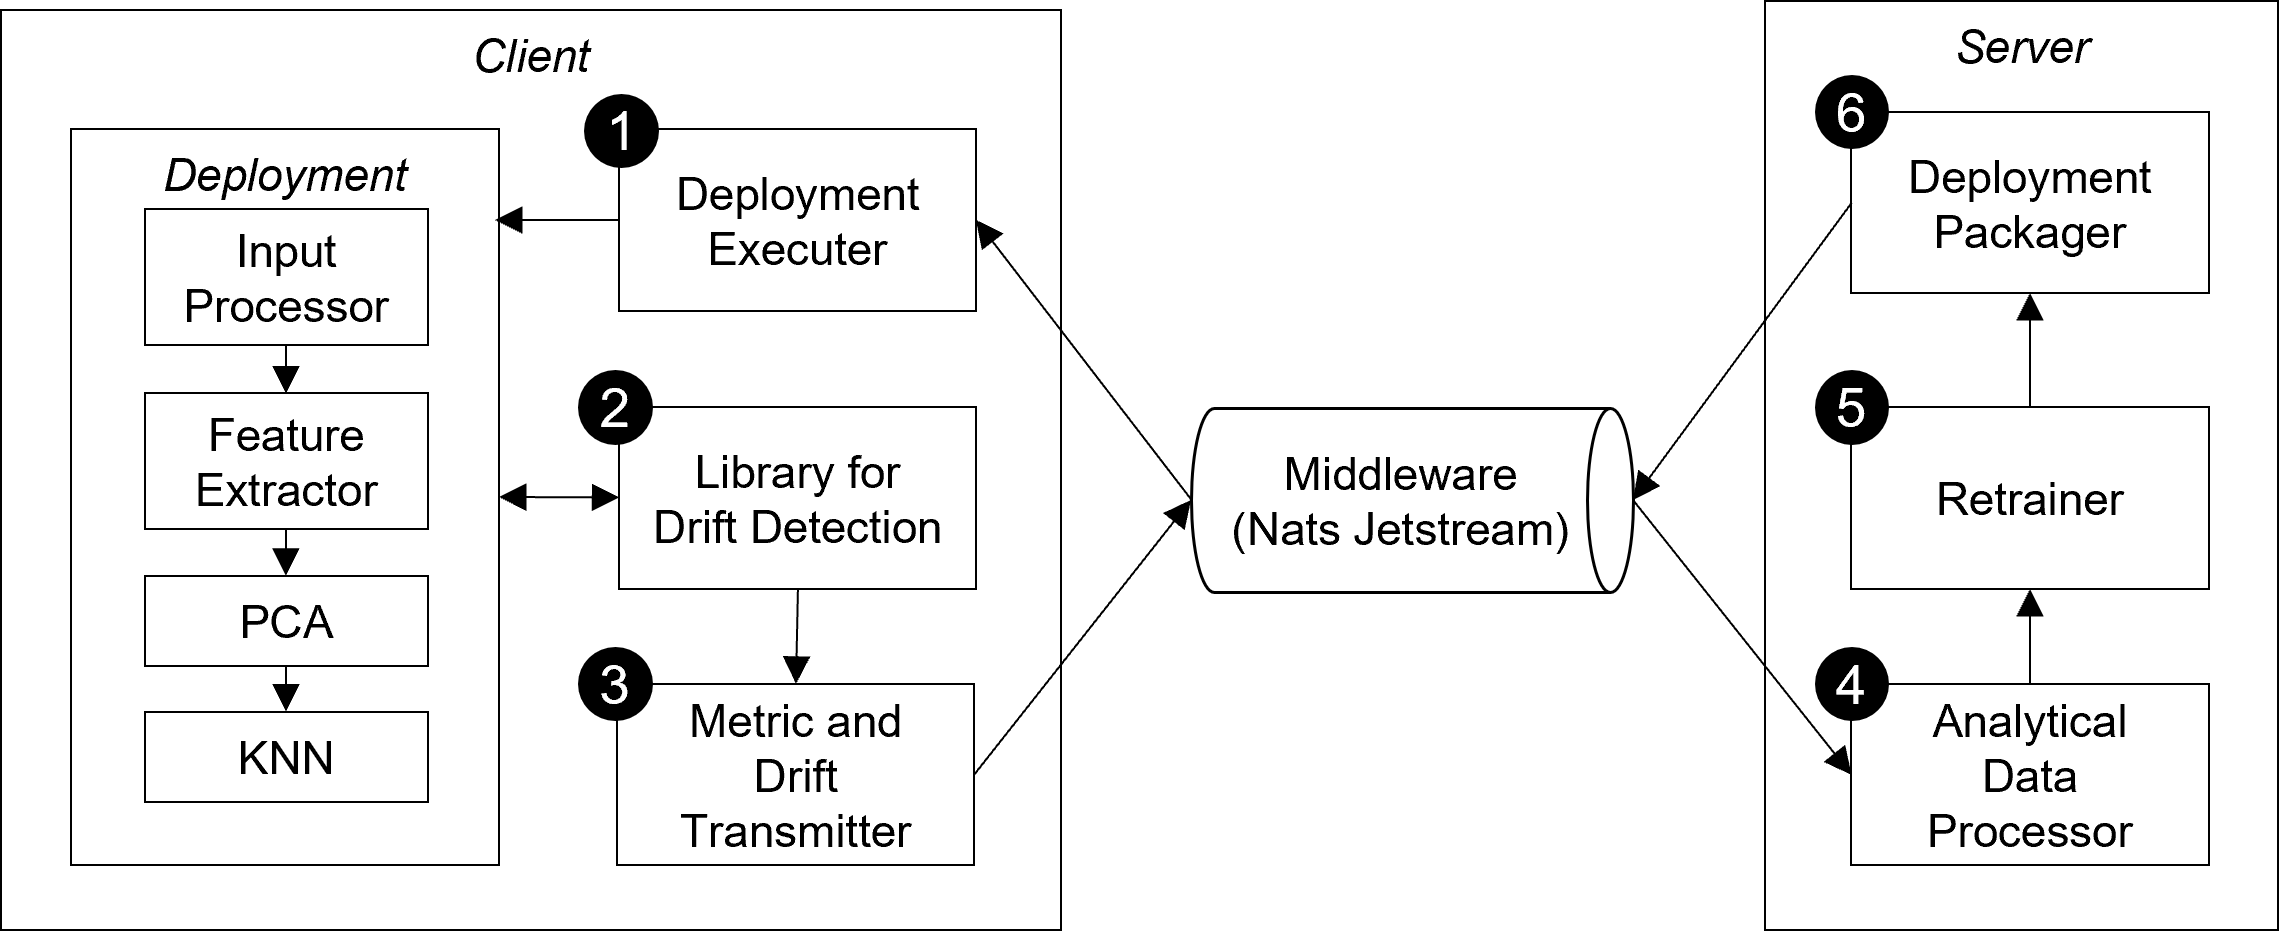
\includegraphics[width=\columnwidth]{Framework-detailed.png}
  \caption{Bird's-eye view of the TinyMLOps framework as documented in the project repository. The client executes the on-device \emph{Deployment} pipeline (Input Processor $\rightarrow$ Feature Extractor $\rightarrow$ PCA $\rightarrow$ distance-based classifier), drift detection, and metric transmission. The server performs analytical processing, retraining, and deployment packaging, while a NATS JetStream middleware connects both sides.}
  \Description{Block diagram of the TinyMLOps framework showing the client deployment pipeline, drift detection, metric transmitter, the NATS JetStream middleware, and the server-side analytical data processor, retrainer, and deployment packager.}
  \label{fig:framework}
\end{figure}

\subsection{Model Architecture and Inference Pipeline}
\label{sec:model-arch}
The on-device inference pipeline consists of several components that run before the distance-based classifier.
The \emph{Input Processor} loads an image and applies the preprocessing that matches the exported model, i.e.\ resizing and pixel normalization.
The \emph{Feature Extractor} is a convolutional neural network exported as an INT8 TensorFlow Lite model that maps the preprocessed image to a fixed-length feature vector.
The extracted feature vector is then standardized and, in the PCA variants, projected onto a lower-dimensional subspace.
Only the final, optionally PCA-reduced feature vector is passed to the distance-based classifier (KNN, Nearest Centroid, or KMeans), which produces the class prediction.

The two dataset families use different feature extractors.
For CIFAR-10, a compact low-resolution MobileNet-style network~\cite{yuan2022lowres} is trained from scratch on the 32$\times$32 images and produces a 160-dimensional feature vector.
For Imagenette, an ImageNet-pretrained MobileNetV2 backbone~\cite{sandler2018mobilenetv2} is used with 224$\times$224 input images and produces a 1280-dimensional feature vector.
In both cases, the softmax classification head is only used during training of the backbone; the deployed artifact is the feature extractor, and the distance-based classifier replaces the softmax head at inference time~\cite{shima2018augmentation,ravaglia2021tinyml}.
The standardization and PCA parameters are stored together as a feature processor and applied on the device, so that the same transformation is used consistently during benchmarking and would also be used during a future on-device learning step.

The framework can execute KNN, k-means-based classification, and nearest centroid classification by exchanging only the classifier component while keeping the feature extractor and feature processor fixed.
These three methods were selected because they represent distinct points on the same reference-representation spectrum, ranging from exemplar-based storage to increasingly compressed prototype-based storage.
This spectrum is directly aligned with the central TinyML trade-off considered in this work: retaining more reference information can improve classification quality, but it also increases the state that must be stored and searched on the device~\cite{disabato2020incremental,ravaglia2021tinyml}.
Prototype and nearest-mean representations are also well established in few-shot and class-incremental learning, where compact class summaries or selected exemplars are used to support adaptation under memory constraints~\cite{snell2017prototypical,rebuffi2017icarl,mai2021supervised,diao2021generalized}.

KNN is included as the uncompressed exemplar-based baseline.
It keeps labeled feature vectors and classifies a query from the labels of nearby stored samples~\cite{cover1967nearest}.
In an incremental on-device setting, this is the most direct update mechanism: a newly labeled observation can be inserted into the reference store without retraining the feature extractor or solving an optimization problem~\cite{disabato2020incremental}.
For the present study, KNN therefore makes the effect of the number of stored reference samples especially transparent.
At the same time, it exposes the upper-cost side of the design space, because both the reference-store footprint and the brute-force neighborhood search grow with the number of stored samples.

K-means-based classification is included as an intermediate compression strategy.
Instead of retaining every selected exemplar, it summarizes regions of the embedding space by a small number of centroids per class.
This follows the standard k-means objective of choosing cluster centers that minimize within-cluster squared distances, typically optimized by Lloyd-style iterative refinement~\cite{lloyd1982least,kanungo2002efficient}; the broader clustering literature treats k-means as a canonical prototype-based summarization method~\cite{jain2010clustering}.
In this benchmark, k-means therefore tests whether several prototypes per class can preserve much of the accuracy of exemplar storage while reducing the classifier state that must be deployed.

Nearest Centroid is included as the most compact prototype-based baseline.
It stores one centroid per class and assigns a query to the class with the nearest centroid~\cite{calafiore2019sparse,manning2008introduction}.
This design has minimal classifier-state growth with respect to the reference sample count once the class centroid has been computed, and nearest-class-mean variants remain relevant in online class-incremental learning~\cite{mai2021supervised}.
It therefore provides a lower-footprint reference point for evaluating how much accuracy is lost, or retained, when each class is represented by a single prototype.
Together, KNN, k-means, and Nearest Centroid allow the study to separate the influence of algorithmic representation from the influence of sample count and PCA, which is the basis for the three research questions.

\section{Research Design}
\label{sec:design}
This section describes the research design used to answer the research questions.
Each experiment runs through the TinyMLOps framework and varies one or more architectural parameters while keeping the remaining measurement setup constant.
The design follows the three research questions directly: RQ1 varies the classifier, RQ2 varies the number of stored reference samples per class, and RQ3 compares the same configurations with and without PCA.
To keep the description reproducible, the following subsections document what was trained and how (Section~\ref{sec:training}), what was measured and how (Sections~\ref{sec:scope}--\ref{sec:measurement}), and how the collected values were aggregated and analyzed (Section~\ref{sec:analysis}).

\subsection{Benchmark Scope}
\label{sec:scope}
The benchmark evaluates three distance-based classifiers: KMeans, KNN, and Nearest Centroid~\cite{cover1967nearest,kanungo2002efficient,calafiore2019sparse}.
For each classifier, two preprocessing variants are considered: \texttt{nopca}, which uses the full feature representation, and \texttt{pca95var}, which projects features to enough principal components to retain approximately 95\% of the variance.
This variant follows the established PCA practice of selecting the retained dimensionality by a cumulative explained-variance criterion~\cite{jolliffe2002pca}.
Concretely, the retained dimensionality is chosen as the smallest number of principal components whose cumulative explained variance reaches approximately 95\%, following the common recommendation to keep the number of dimensions that add up to a sufficiently large portion of the variance, e.g.\ 95\%~\cite[p.~223]{geron2019handson}.
This threshold is used as a conservative, reproducible operating point: it preserves most of the measured feature-space variance while still reducing the deployed reference vectors, and its practical effect is evaluated directly against the corresponding \texttt{nopca} baseline.
The number of stored reference samples per class is swept over 12 values: 2, 5, 10, 20, 30, 40, 50, 60, 70, 80, 90, and 100.
Each configuration is repeated with ten initialization and test-order seeds: 42, 123, 456, 789, 1337, 1618, 2021, 2718, 3141, and 9876.
This results in 720 completed runs per dataset family, because each dataset combines three classifiers, two PCA settings, 12 sample-count settings, and ten seeds; across both dataset families, 1440 runs were completed.

The classifier configurations are fixed across the sweep.
KNN uses $k=3$ with a Euclidean distance metric and inverse-distance weighting (power 3.0); KMeans uses three prototypes per class; and Nearest Centroid stores one centroid per class.
Only the runtime-specific fields (PCA on/off, maximum reference samples, and the shuffle seed) are patched per experiment, while the classifier type and image resolution are defined by the scenario configuration.

\subsection{Datasets and Feature Representations}
The evaluation uses two image-classification benchmark families.
CIFAR-10~\cite{krizhevsky2009cifar} is used as a low-resolution benchmark with 32$\times$32 input images and ten classes.
Its extracted feature representation has 160 dimensions without PCA and 31 dimensions with \texttt{pca95var}, retaining 95.14\% of the variance.
Imagenette, a ten-class subset of ImageNet~\cite{deng2009imagenet,howard2019imagenette}, is used as a higher-resolution benchmark with 224$\times$224 input images.
The choice of CIFAR-10 and Imagenette follows common practice in the small-data image-classification literature, where most studies rely on sub-sampled versions of standard benchmarks such as CIFAR and ImageNet~\cite{brigato2022small}; Imagenette in particular remains in active use as a benchmark in recent CNN evaluations~\cite{saberifard2025xtorch}.
Its extracted feature representation has 1280 dimensions without PCA and 608 dimensions with \texttt{pca95var}, retaining 95.02\% of the variance.
For both dataset families, the scenario-level feature processing and PCA preparation use the corresponding training split.
The deployed distance-based classifier is then initialized from a sampled reference store whose size is controlled by the samples-per-class setting; benchmark test images are evaluated separately from this sampled reference store.

The benchmark keeps the reference-store construction and the measured test set separate at the directory level.
For CIFAR-10, the repository export script writes the official CIFAR-10 training batches to the dataset's \texttt{train} directory and the official test batch to its \texttt{test} directory.
For Imagenette, the export uses the Imagenette training split as the training/reference directory and maps Imagenette's validation split to the benchmark \texttt{test} directory.
Initial classifier states are built only from the corresponding \texttt{train} directory of the dataset family.
For a given seed and class index, the initial-state script first sorts the available class images, then draws at most the configured number of samples per class without replacement using a class-specific generator seeded by the run seed plus the class index.
The selected images are converted to feature vectors with the same TensorFlow Lite feature extractor and optional feature processor that are deployed on the device.
KNN stores the selected feature vectors directly, whereas Nearest Centroid and KMeans fit their prototypes from exactly the same selected per-class reference set; the selected indices and per-class counts are persisted in the initial-state metadata.

The benchmark test set for each deployment is rebuilt from the corresponding held-out \texttt{test} directory before packaging the scenario.
The pipeline deletes and recreates the scenario's deployment image directory, iterates over the sorted class folders, shuffles each class with the same class-specific seed rule, and copies the first configured test images into the deployment package.
With 20 test images per class and ten classes, each run therefore evaluates exactly 200 benchmark test images, balanced as 20 images per class.
Because the same seed is used for both reference sampling and test-image selection, one run is reproducible end-to-end; because ten different seeds are used, the reported means aggregate over different reference stores and different class-balanced subsets of the held-out test split.

\subsection{Model Training and Architecture Creation}
\label{sec:training}
The feature extractor and the feature processor are created once per dataset family and then reused unchanged across all three classifier scenarios of that dataset.
In other words, KNN, KMeans, and Nearest Centroid for a given dataset share exactly the same feature extractor and the same PCA projection, so that differences between them are attributable to the classifier rather than to a different backbone.
The backbones are trained with a fixed seed of 42 and a validation split of 0.2.
The CIFAR-10 low-resolution MobileNet is trained from scratch on the CIFAR-10 training split for 20 epochs, and the Imagenette backbone fine-tunes a pretrained MobileNetV2 (10 initial training epochs followed by 5 fine-tuning epochs).
The backbones are then exported as INT8 TensorFlow Lite feature extractors and mirrored into the three classifier scenarios; INT8 quantization is known to retain accuracy well on standard image benchmarks~\cite{shabir2025compression,ravaglia2021tinyml}.
The benchmark itself does not retrain the backbone: it trains the pipeline on the full training split once and only varies the initialization reference-sample size on the device.

Table~\ref{tab:backbone-training-stats} summarizes the available backbone training statistics.
For CIFAR-10, the final epoch of the 20-epoch low-resolution MobileNet training run reached 0.8211 training accuracy and 0.8113 validation accuracy.
For Imagenette, a reproduced run with the same seed and configuration reached 0.9688 training accuracy and 0.9810 validation accuracy after fine-tuning; its best validation accuracy during the run was 0.9905 in the initial training phase.
Because TensorFlow training was not configured for bit-identical determinism, the reproduced Imagenette values should be interpreted as representative of the backbone configuration rather than as exact measurements of the originally deployed TFLite artifact.

\begin{table*}[t]
  \caption{Backbone training statistics before exporting the feature extractors. CIFAR-10 reports the final epoch of the original 20-epoch low-resolution MobileNet run; Imagenette reports a reproduced run with the same seed and training configuration.}
  \label{tab:backbone-training-stats}
  \centering
  \footnotesize
  \begin{tabular}{@{}llllrrrr@{}}
    \toprule
    Dataset & Backbone & Input & Training setup & Train loss & Train acc. & Val. loss & Val. acc. \\
    \midrule
    CIFAR-10 & Low-res MobileNet & 32$\times$32 & 20 epochs, from scratch & 0.5142 & 0.8211 & 0.5497 & 0.8113 \\
    Imagenette & MobileNetV2 & 224$\times$224 & 10 + 5 epochs, pretrained & 0.0919 & 0.9688 & 0.0679 & 0.9810 \\
    \bottomrule
  \end{tabular}
\end{table*}

The PCA configuration is a deliberate design choice rather than an incidental result.
For the \texttt{pca95var} variants, the number of retained components is selected by cumulative explained variance, which is a standard PCA criterion for dimensionality selection~\cite{jolliffe2002pca}.
The threshold is set to approximately 95\%, following the widely used recommendation to retain enough principal components to preserve on the order of 95\% of the variance when reducing dimensionality~\cite[p.~223]{geron2019handson}, as a conservative operating point rather than as a theoretically optimal constant.
This choice avoids an aggressive compression of the learned embedding, keeps most of the measured variance, and still creates a measurable reduction in classifier state and reference-store size.
Its practical effect is not assumed from the threshold alone; it is evaluated explicitly by comparing every \texttt{pca95var} configuration with the corresponding no-PCA baseline in terms of accuracy, latency, energy, process memory, and classifier/reference-store footprint.
With this target, the PCA fitted on the CIFAR-10 features selects 31 components and retains 95.14\% of the variance, and the PCA fitted on the Imagenette features selects 608 components and retains 95.02\% of the variance.
The feature processor (standardization mean and scale together with the PCA projection matrix) is stored as a single artifact and applied identically on the device.
The reported classifier-state sizes in the result tables do not include this fixed feature-processor artifact; they measure only the active distance-based classifier and its stored reference vectors or prototypes.
Table~\ref{tab:feature-processor-overhead} therefore reports the feature-processor overhead separately.
The runtime artifact stores three \texttt{float32} arrays: the scaler mean, the inverse scaler standard deviation, and the PCA projection matrix.
Consequently, its payload size is approximately $(2D + dD)\cdot4$ bytes for input dimension $D$ and PCA output dimension $d$, plus a small \texttt{npz} container overhead.

\begin{table}[t]
  \caption{Stored feature-processor overhead for the \texttt{pca95var} variants. The artifact contains the standardization parameters and PCA projection matrix and is separate from the classifier state reported in Tables~\ref{tab:sweet-spots-eff} and~\ref{tab:pca-effect}.}
  \label{tab:feature-processor-overhead}
  \centering
  \footnotesize
  \begin{tabular}{@{}lrrrr@{}}
    \toprule
    Dataset & Input dim. & PCA dim. & Array payload & NPZ file \\
    \midrule
    CIFAR-10 & 160 & 31 & 20.63~KB & 22.13~KB \\
    Imagenette & 1280 & 608 & 3050.00~KB & 3052.06~KB \\
    \bottomrule
  \end{tabular}
\end{table}

\subsection{Data Collection Procedures}
\label{sec:measurement}
All resource measurements are collected on a Raspberry Pi Zero 2W.
The device is powered by a Voltcraft DSP-3005 external power supply at 5~V, and the external power log is integrated per experiment to obtain the energy consumed during that run.
Each experiment corresponds to a bounded on-device measurement window that covers the classification of that run's 200 test images and over which the resource and power logs are recorded.
This window lasted about 49~s per run on CIFAR-10 and about 116~s on Imagenette (overall range roughly 49--124~s across the 1440 deployments), while the mean per-image inference latency was about 45~ms on CIFAR-10 and 356~ms on Imagenette, with the remaining per-image time spent on image loading and preprocessing.
The window length is therefore set almost entirely by the shared feature extraction and preprocessing rather than by the lightweight distance-based classifier, so it barely varies across classifiers or sample-count settings but differs clearly between the two datasets.
For each deployed configuration, the pipeline records classification accuracy, per-image latency, CPU usage, and resident-set-size (RSS) memory from the merged benchmark and resource logs written on the device.
In addition, it records the analytical classifier state size and reference-store size, so that memory is represented both as observed process memory and as model-specific storage demand.
These storage metrics are the active classifier/reference-store indicators that grow directly with the number of stored reference samples and with the feature dimensionality; the fixed PCA feature-processor artifact is reported separately in Table~\ref{tab:feature-processor-overhead}.
Gross power and energy are derived from the external supply metadata, while net power and net energy subtract a separately measured idle baseline of the device, so that the reported net values approximate the additional cost caused by the inference workload.
All energy measurements were taken under single-threaded BLAS/OpenMP execution, so that multi-threaded PCA projection could not distort the energy comparison across configurations. For CIFAR-10, the small 31-dimensional PCA projection never engaged OpenBLAS multi-threading, so those runs were single-threaded regardless. For Imagenette, the larger 608-dimensional projection did: an earlier, non-pinned run showed an inflated PCA energy figure that was traced to OpenBLAS multi-threading and corrected by explicitly pinning BLAS/OpenMP to one thread and re-running the experiments.

\subsection{Data Analysis Procedures}
\label{sec:analysis}
For every configuration, the ten seeds are summarized by their mean; the reported mean accuracy and mean resource metrics are therefore averages over the ten seeds.
Dispersion across seeds is reported as the standard deviation and as the 95\% confidence interval (CI) of the mean.
Unless stated otherwise, the reported ``95\% CI'' value is the half-width of the 95\% confidence interval of the seed mean, computed with the t-distribution and $n-1$ degrees of freedom; a reported value of, for example, 0.0152 therefore means the seed mean lies within $\pm$0.0152 with 95\% confidence.
The dependent variables capture the resulting accuracy--efficiency trade-off: classification accuracy, latency, CPU usage, RSS memory, analytical classifier/reference-store size, fixed feature-processor overhead, net average power, and net energy per image.

For RQ1, configurations are compared by the best observed mean accuracy per classifier and PCA setting together with their resource behavior.
For RQ2, the sweet spot is operationalized as the first sample-count setting that reaches at least 95\% (or 99\%) of the maximum observed mean accuracy of the same dataset, classifier, and PCA configuration; the corresponding accuracy and efficiency metrics at that knee are reported alongside the sample count.
For RQ3, PCA influence is measured as paired \texttt{pca95var} minus \texttt{nopca} differences where matching configurations exist, across accuracy, energy, and the storage-footprint metrics.
Paired Wilcoxon signed-rank tests are computed in the analysis exports for the PCA comparisons as a robustness check, but the main paper focuses on effect size and practical deployment relevance.

\section{Results}
\label{sec:results}
The results are based on the most recent export folders available for both benchmark families: \texttt{analysis\_20260713\_083731} for CIFAR-10 and \texttt{analysis\_20260713\_083731} for Imagenette (the thread-pinned re-run).
Figure~\ref{fig:cifar10-summary-grid} provides the CIFAR-10 benchmark overview and Figure~\ref{fig:imagenet-summary-grid} the Imagenette benchmark overview.
Figure~\ref{fig:cifar10-energy-samples} and Figure~\ref{fig:imagenet-energy-samples} show the dataset-specific energy behavior, and Figure~\ref{fig:imagenet-ram-usage} visualizes the strongest observed reference-store effect in process memory.
The following subsections answer the research questions in detail.

\begin{figure*}[t]
  \centering
  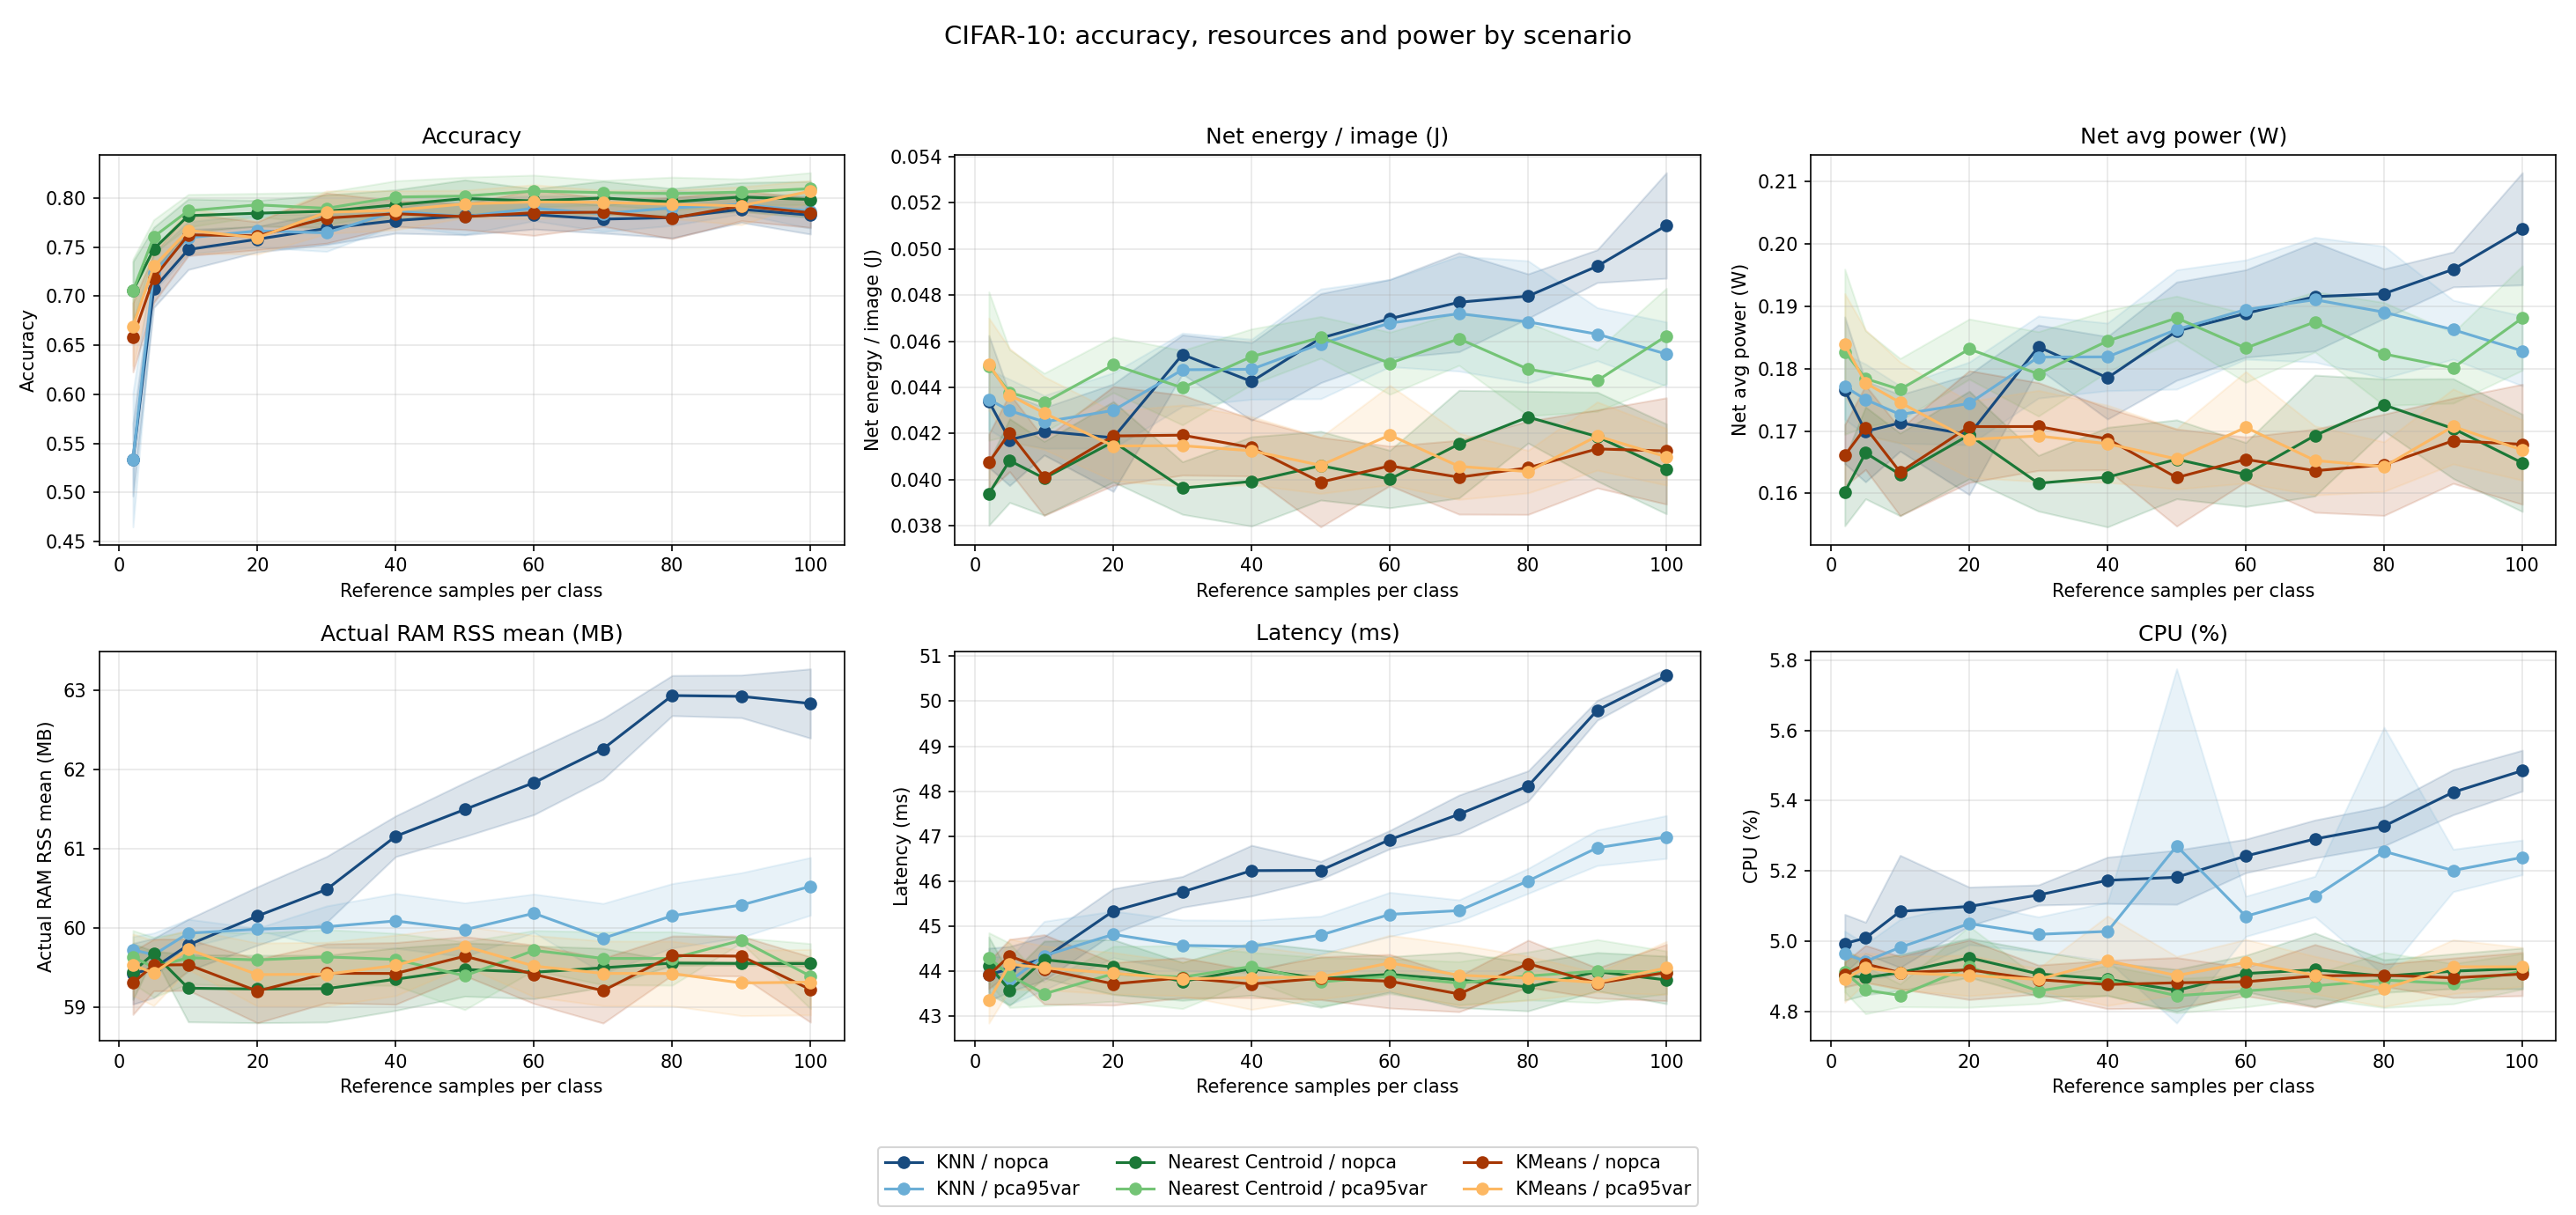
\includegraphics[width=\textwidth]{cifar10_summary_grid.png}
  \caption{CIFAR-10 benchmark overview across the reference-sample sweep. The panels report mean accuracy, net energy per image, net average power, mean process RSS, latency, and CPU utilization for each classifier/PCA combination; shaded bands denote 95\% confidence intervals across the ten seeds. Accuracy saturates early, whereas KNN without PCA shows the strongest increase in memory, latency, and energy as the reference store grows.}
  \Description{Six-panel CIFAR-10 benchmark summary showing accuracy, net energy per image, net average power, mean process RSS, latency, and CPU utilization across reference-sample counts for KMeans, KNN, and Nearest Centroid with and without PCA.}
  \label{fig:cifar10-summary-grid}
\end{figure*}

\begin{figure*}[t]
  \centering
  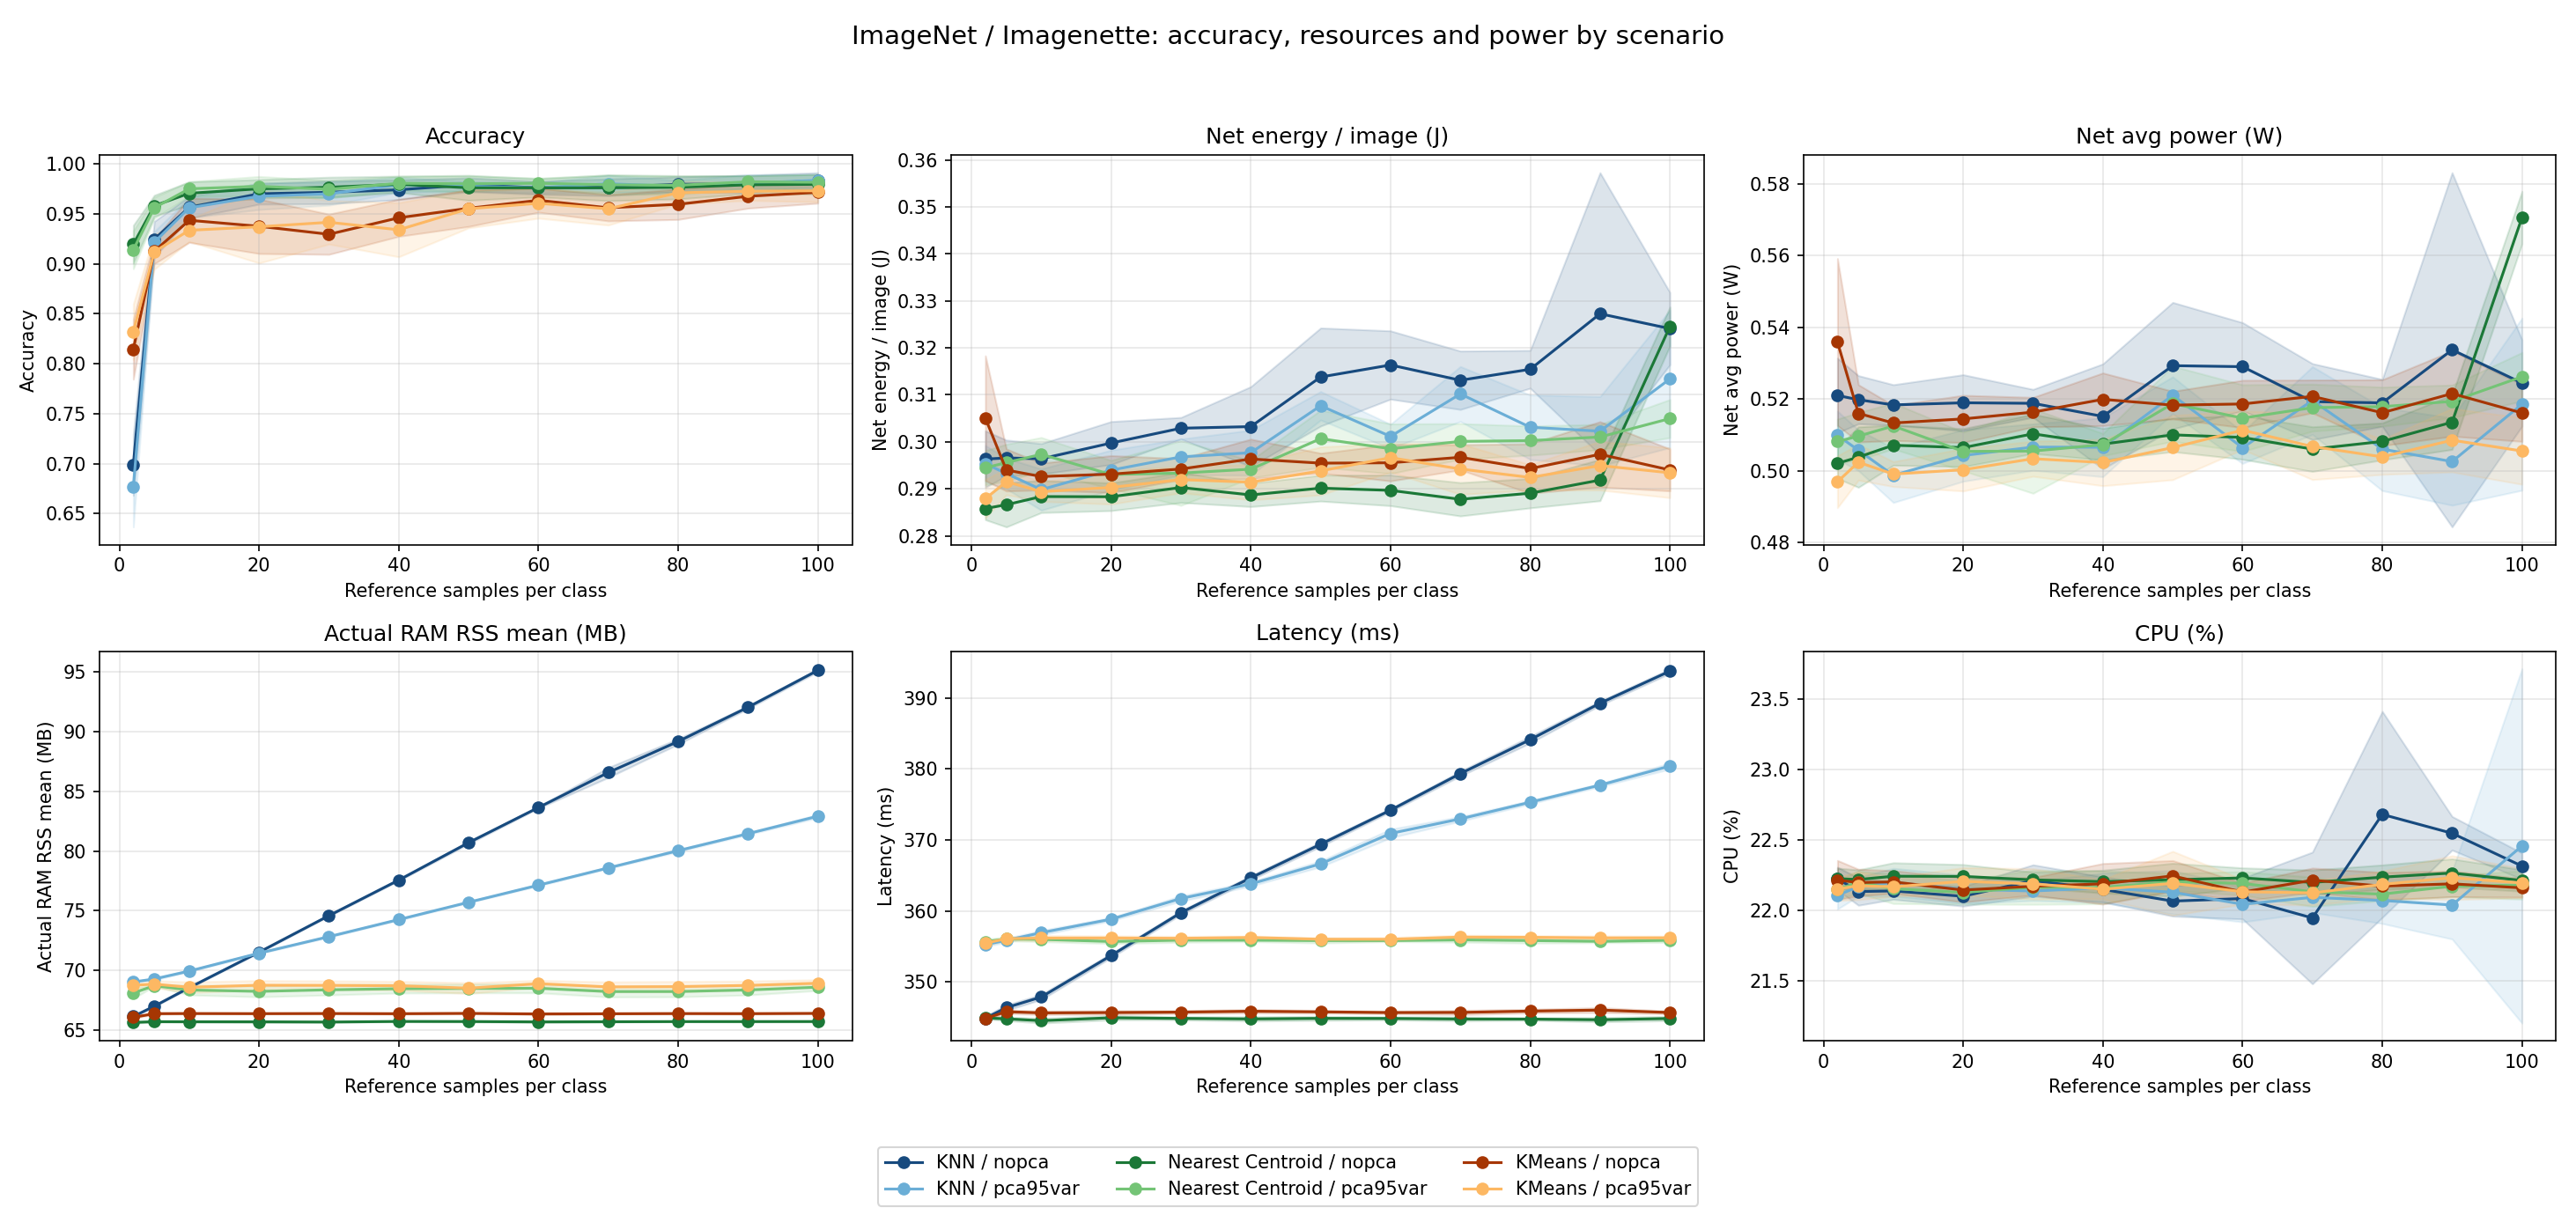
\includegraphics[width=\textwidth]{imagenet_summary_grid.png}
  \caption{Imagenette benchmark overview across the reference-sample sweep. The panels report mean accuracy, net energy per image, net average power, mean process RSS, latency, and CPU utilization for each classifier/PCA combination; shaded bands denote 95\% confidence intervals across the ten seeds. KNN reaches the highest accuracy but also exhibits the clearest sample-count-dependent increase in process memory and latency, while the prototype-based classifiers remain nearly flat in these resource metrics.}
  \Description{Six-panel Imagenette benchmark summary showing accuracy, net energy per image, net average power, mean process RSS, latency, and CPU utilization across reference-sample counts for KMeans, KNN, and Nearest Centroid with and without PCA.}
  \label{fig:imagenet-summary-grid}
\end{figure*}

\begin{figure*}[t]
  \centering
  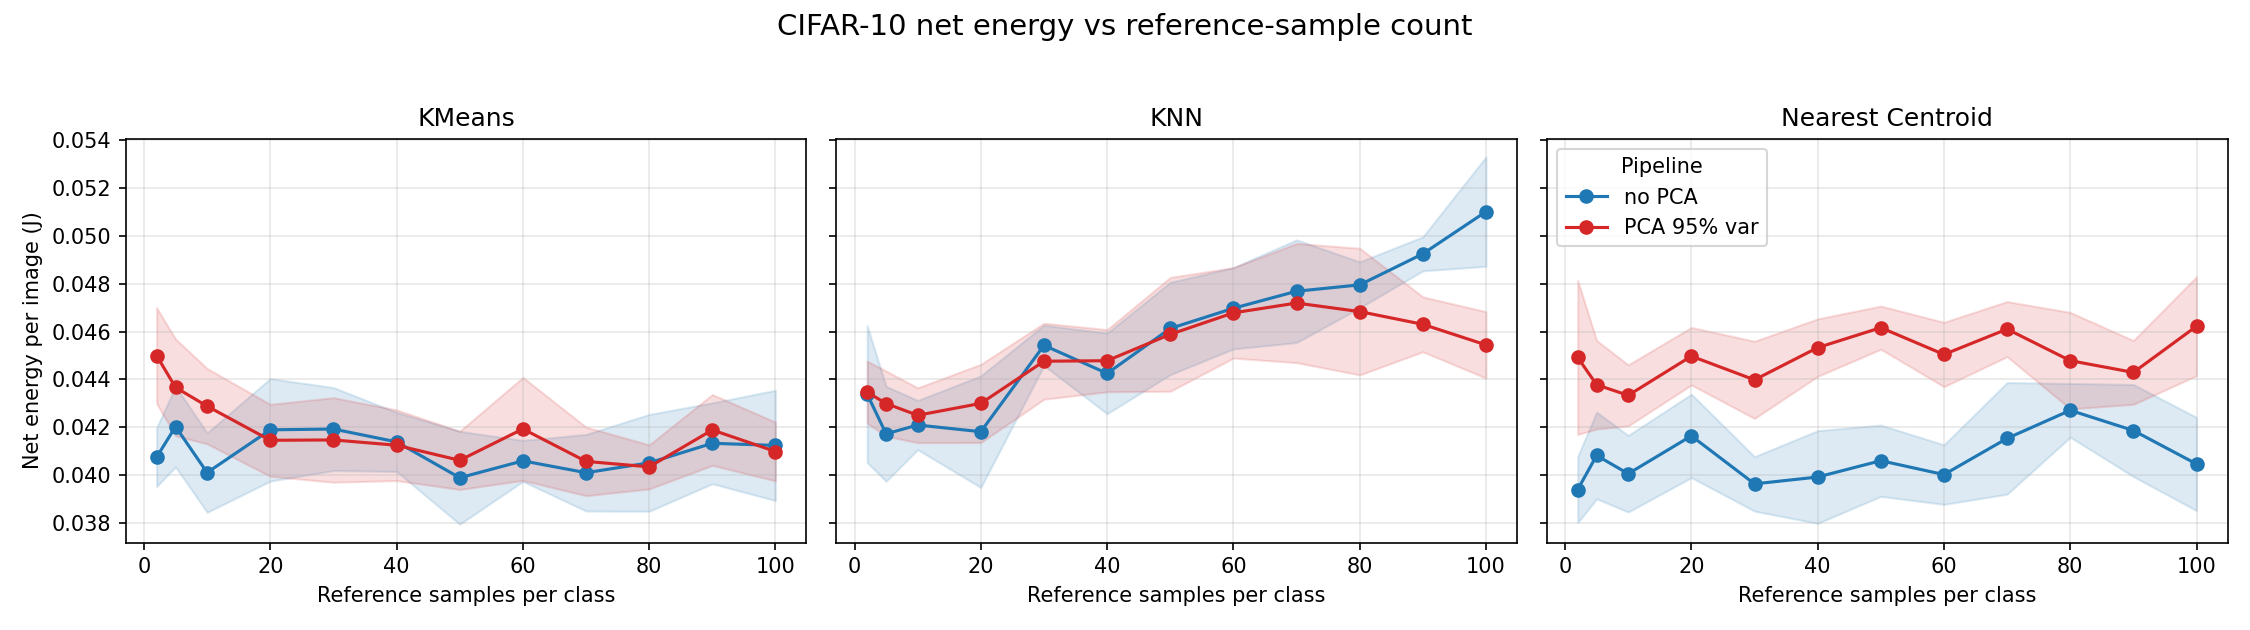
\includegraphics[width=\textwidth]{cifar10_energy_vs_samples.png}
  \caption{CIFAR-10 net energy per image by classifier and reference-sample count. Lines show seed means and shaded bands show 95\% confidence intervals. KMeans remains comparatively stable across the sweep, KNN energy increases with larger reference stores, and Nearest Centroid with \texttt{pca95var} is consistently above its no-PCA counterpart despite the smaller classifier state.}
  \Description{Three CIFAR-10 line plots comparing no-PCA and pca95var net energy per image across reference-sample counts for KMeans, KNN, and Nearest Centroid.}
  \label{fig:cifar10-energy-samples}
\end{figure*}

\begin{figure*}[t]
  \centering
  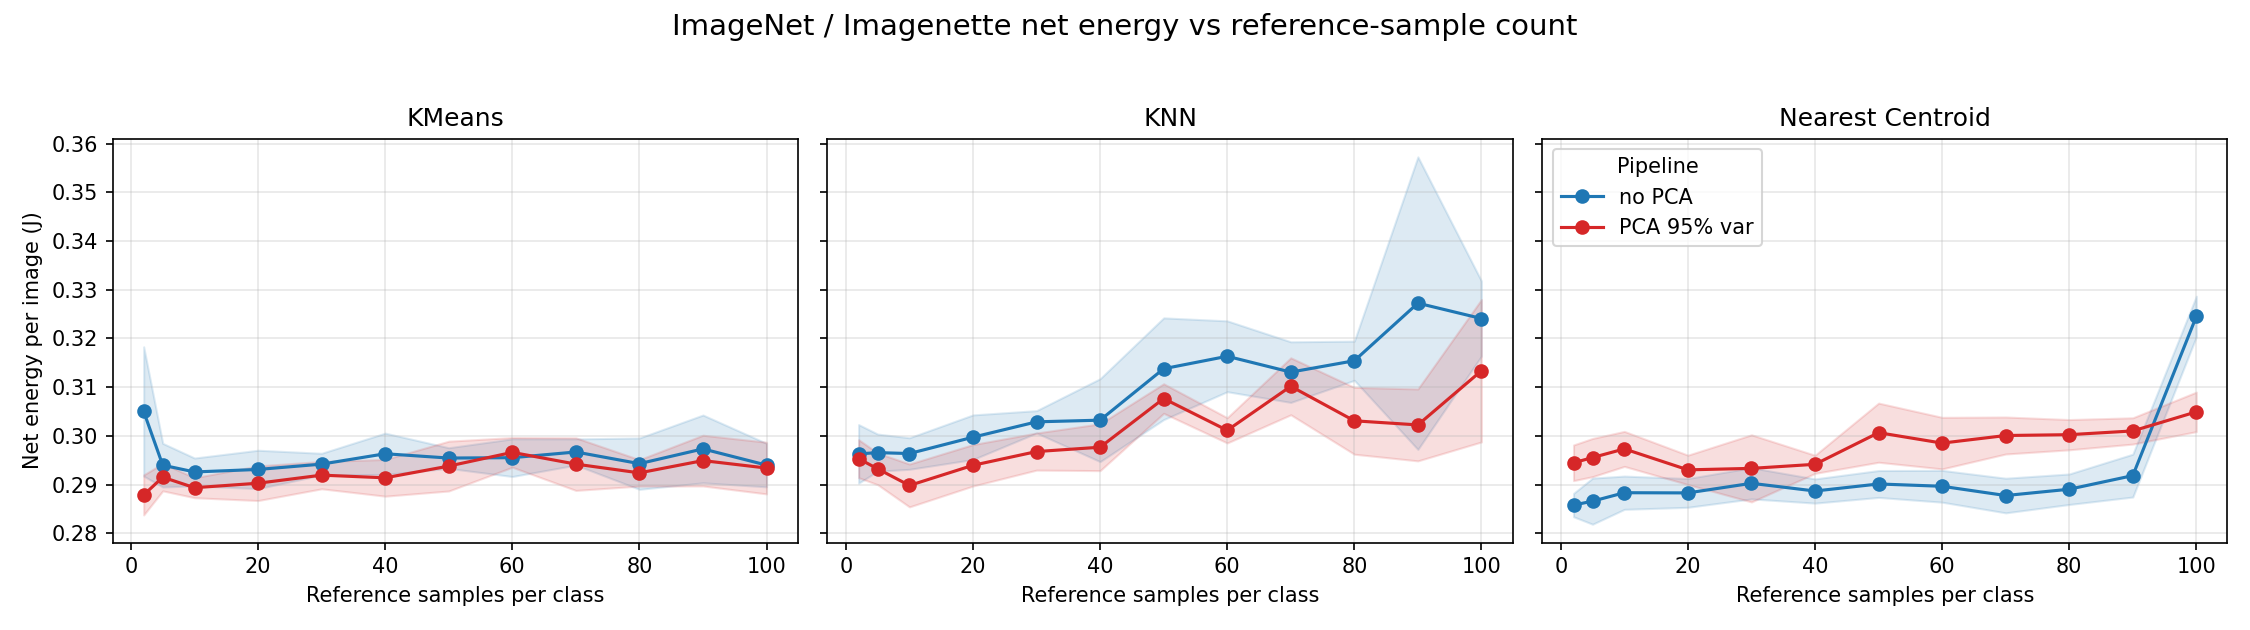
\includegraphics[width=0.94\textwidth]{imagenet_energy_vs_samples.png}
  \caption{Imagenette net energy per image by classifier and reference-sample count in the thread-pinned export. Lines show seed means and shaded bands show 95\% confidence intervals. KMeans shows small PCA--no-PCA differences, KNN tends to consume less energy with \texttt{pca95var} at larger reference stores, and Nearest Centroid shows a small PCA-related increase for most sample counts.}
  \Description{Three Imagenette line plots comparing no-PCA and pca95var net energy per image across reference-sample counts for KMeans, KNN, and Nearest Centroid after the thread-pinned re-run.}
  \label{fig:imagenet-energy-samples}
\end{figure*}

\begin{figure*}[t]
  \centering
  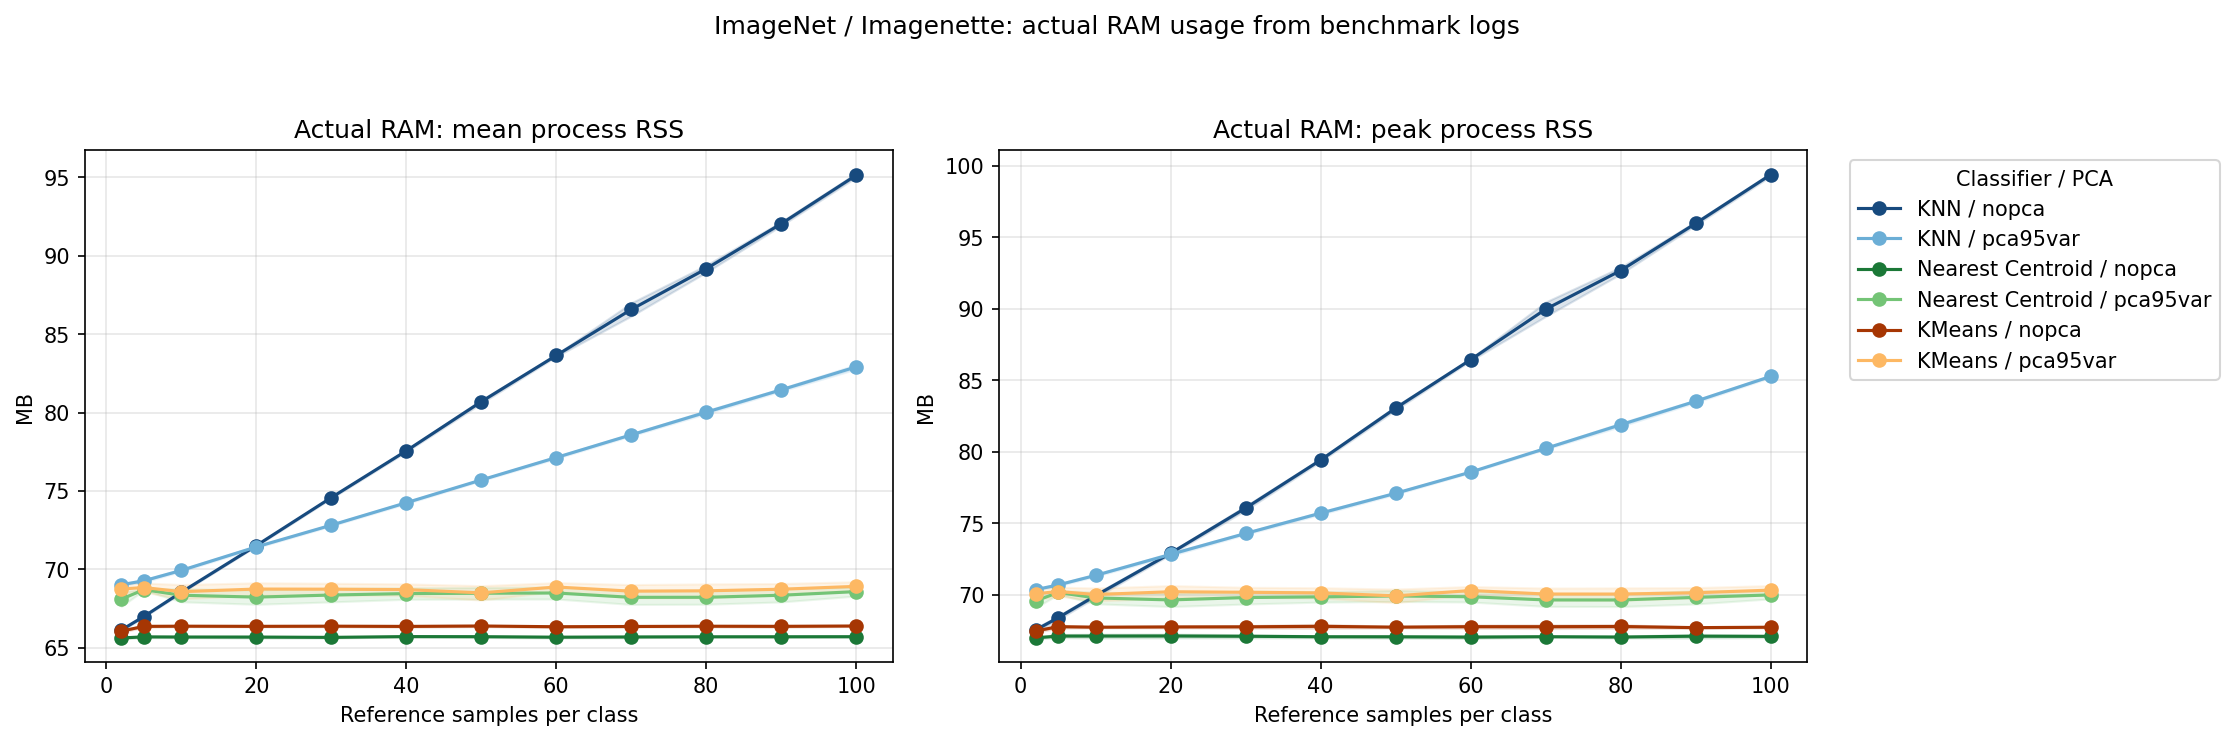
\includegraphics[width=0.94\textwidth]{imagenet_actual_ram_usage.png}
  \caption{Observed Imagenette process memory from the benchmark logs. The panels show mean and peak process RSS across the reference-sample sweep. Memory growth is concentrated in KNN because its reference store grows with the number of stored exemplars; \texttt{pca95var} reduces this slope, while KMeans and Nearest Centroid remain nearly constant.}
  \Description{Two Imagenette line plots showing mean and peak process RSS across reference-sample counts for KMeans, KNN, and Nearest Centroid with and without PCA. KNN without PCA grows most strongly, KNN with PCA grows more slowly, and the prototype-based classifiers remain nearly flat.}
  \label{fig:imagenet-ram-usage}
\end{figure*}

\subsection{RQ1: Algorithm Selection}
Table~\ref{tab:best-accuracy} reports the best observed mean accuracy for each classifier and PCA configuration.
For CIFAR-10, the highest observed mean accuracy is 0.8095 for Nearest Centroid with \texttt{pca95var} at 100 samples per class.
KMeans reaches 0.8070 with \texttt{pca95var} at 100 samples per class, while KNN reaches 0.7935 with \texttt{pca95var} at 90 samples per class.
Without PCA, the best CIFAR-10 mean accuracies are 0.8010 for Nearest Centroid, 0.7920 for KMeans, and 0.7885 for KNN.

For Imagenette, KNN has the highest observed mean accuracy with 0.9835 using \texttt{pca95var} at 100 samples per class and 0.9830 without PCA at 100 samples per class.
Nearest Centroid reaches 0.9820 with \texttt{pca95var} at 90 samples per class and 0.9795 without PCA at 100 samples per class.
KMeans reaches 0.9730 with \texttt{pca95var} and 0.9715 without PCA, both at 100 samples per class.

\begin{table*}[t]
  \caption{Best observed mean accuracy per dataset, classifier, and PCA configuration. The 95\% CI column is the half-width of the 95\% confidence interval of the mean across the ten seeds (t-distribution, $n-1$ df).}
  \label{tab:best-accuracy}
  \centering
  \footnotesize
  \begin{tabular}{@{}lllrrr@{}}
    \toprule
    Dataset & Classifier & PCA & Samples/class & Accuracy mean & 95\% CI \\
    \midrule
    CIFAR-10 & KMeans & nopca & 90 & 0.7920 & 0.0152 \\
    CIFAR-10 & KMeans & pca95var & 100 & 0.8070 & 0.0108 \\
    CIFAR-10 & KNN & nopca & 90 & 0.7885 & 0.0134 \\
    CIFAR-10 & KNN & pca95var & 90 & 0.7935 & 0.0097 \\
    CIFAR-10 & Nearest Centroid & nopca & 90 & 0.8010 & 0.0148 \\
    CIFAR-10 & Nearest Centroid & pca95var & 100 & 0.8095 & 0.0163 \\
    Imagenette & KMeans & nopca & 100 & 0.9715 & 0.0109 \\
    Imagenette & KMeans & pca95var & 100 & 0.9730 & 0.0111 \\
    Imagenette & KNN & nopca & 100 & 0.9830 & 0.0081 \\
    Imagenette & KNN & pca95var & 100 & 0.9835 & 0.0059 \\
    Imagenette & Nearest Centroid & nopca & 100 & 0.9795 & 0.0099 \\
    Imagenette & Nearest Centroid & pca95var & 90 & 0.9820 & 0.0064 \\
    \bottomrule
  \end{tabular}
\end{table*}

The resource summaries show that CIFAR-10 mean net energy per image ranges from 0.0407~J for Nearest Centroid without PCA to 0.0456~J for KNN without PCA.
The corresponding mean latency values range from 43.87~ms for KMeans without PCA to 46.56~ms for KNN without PCA.
For Imagenette without PCA, mean net energy per image ranges from 0.2918~J for Nearest Centroid to 0.3088~J for KNN.
With \texttt{pca95var}, the Imagenette mean net energy per image ranges from 0.2923~J for KMeans to 0.3004~J for KNN.
The corresponding Imagenette PCA net power values are approximately 0.50--0.51~W, comparable to the no-PCA range of approximately 0.51--0.52~W.
Table~\ref{tab:resource-summary} summarizes these resource measurements together with latency and observed RSS memory.

\subsection{RQ2: Reference Sample Sweet Spot}
Table~\ref{tab:sweet-spots} reports the reference-sample knees using two thresholds: the first number of samples per class that reaches at least 95\% of the maximum observed mean accuracy, and the corresponding number for 99\%.
For each knee, the table also reports the mean accuracy actually reached at that sample count, so that the operating point can be read directly.
For CIFAR-10 at the 95\% threshold, KMeans reaches the knee at 10 samples per class (accuracy 0.7625) with and without PCA.
KNN reaches the 95\% knee at 20 samples per class (0.7580) without PCA and at 10 (0.7595) with \texttt{pca95var}.
Nearest Centroid reaches the 95\% knee at 10 samples per class in both PCA settings (0.7820 without PCA, 0.7870 with PCA).

For Imagenette at the 95\% threshold, KMeans and KNN reach the knee at 10 samples per class in both PCA settings, and Nearest Centroid reaches it already at 5 samples per class with and without PCA (0.9580 without PCA, 0.9560 with PCA).
At the stricter 99\% threshold, CIFAR-10 knees range from 40 to 100 samples per class, while Imagenette knees range from 10 to 80 samples per class.

Because RQ2 concerns the accuracy--efficiency trade-off and not only the sample count, Table~\ref{tab:sweet-spots-eff} additionally reports the efficiency metrics measured at the 95\% knee: net energy per image, latency, RSS memory, and the active classifier state size.
The classifier state size at the knee makes the reference-store footprint explicit and already previews the PCA effect analyzed in RQ3: at the same knee, the \texttt{pca95var} state is consistently smaller than the \texttt{nopca} state (for example, Imagenette KNN drops from 500~KB to 237.5~KB, and CIFAR-10 Nearest Centroid from 6.25~KB to 1.21~KB), while energy and latency remain close.

\begin{table*}[t]
  \caption{Reference-sample knees at 95\% and 99\% of the maximum observed mean accuracy, with the mean accuracy actually reached at each knee.}
  \label{tab:sweet-spots}
  \centering
  \footnotesize
  \begin{tabular}{@{}lllrrrrr@{}}
    \toprule
    Dataset & Classifier & PCA & Max accuracy & 95\% knee & Acc.\ @95\% & 99\% knee & Acc.\ @99\% \\
    \midrule
    CIFAR-10 & KMeans & nopca & 0.7920 & 10 & 0.7625 & 60 & 0.7850 \\
    CIFAR-10 & KMeans & pca95var & 0.8070 & 10 & 0.7670 & 100 & 0.8070 \\
    CIFAR-10 & KNN & nopca & 0.7885 & 20 & 0.7580 & 50 & 0.7820 \\
    CIFAR-10 & KNN & pca95var & 0.7935 & 10 & 0.7595 & 40 & 0.7865 \\
    CIFAR-10 & Nearest Centroid & nopca & 0.8010 & 10 & 0.7820 & 40 & 0.7930 \\
    CIFAR-10 & Nearest Centroid & pca95var & 0.8095 & 10 & 0.7870 & 50 & 0.8020 \\
    Imagenette & KMeans & nopca & 0.9715 & 10 & 0.9435 & 60 & 0.9635 \\
    Imagenette & KMeans & pca95var & 0.9730 & 10 & 0.9335 & 80 & 0.9710 \\
    Imagenette & KNN & nopca & 0.9830 & 10 & 0.9565 & 40 & 0.9740 \\
    Imagenette & KNN & pca95var & 0.9835 & 10 & 0.9560 & 40 & 0.9790 \\
    Imagenette & Nearest Centroid & nopca & 0.9795 & 5 & 0.9580 & 10 & 0.9705 \\
    Imagenette & Nearest Centroid & pca95var & 0.9820 & 5 & 0.9560 & 10 & 0.9750 \\
    \bottomrule
  \end{tabular}
\end{table*}

\begin{table*}[t]
  \caption{Efficiency metrics measured at the 95\% accuracy knee of Table~\ref{tab:sweet-spots}. State size is the analytical active classifier/reference-store state at the knee sample count and excludes the fixed feature-processor artifact listed in Table~\ref{tab:feature-processor-overhead}.}
  \label{tab:sweet-spots-eff}
  \centering
  \footnotesize
  \begin{tabular}{@{}lllrrrrr@{}}
    \toprule
    Dataset & Classifier & PCA & 95\% knee & Net energy/img (J) & Latency (ms) & RSS (MB) & State (KB) \\
    \midrule
    CIFAR-10 & KMeans & nopca & 10 & 0.0401 & 44.0 & 59.54 & 18.75 \\
    CIFAR-10 & KMeans & pca95var & 10 & 0.0429 & 44.1 & 59.73 & 3.63 \\
    CIFAR-10 & KNN & nopca & 20 & 0.0418 & 45.3 & 60.15 & 125.00 \\
    CIFAR-10 & KNN & pca95var & 10 & 0.0425 & 44.3 & 59.94 & 12.11 \\
    CIFAR-10 & Nearest Centroid & nopca & 10 & 0.0401 & 44.2 & 59.24 & 6.25 \\
    CIFAR-10 & Nearest Centroid & pca95var & 10 & 0.0433 & 43.5 & 59.63 & 1.21 \\
    Imagenette & KMeans & nopca & 10 & 0.2926 & 345.7 & 66.38 & 150.00 \\
    Imagenette & KMeans & pca95var & 10 & 0.2894 & 356.2 & 68.58 & 71.25 \\
    Imagenette & KNN & nopca & 10 & 0.2964 & 347.9 & 68.54 & 500.00 \\
    Imagenette & KNN & pca95var & 10 & 0.2898 & 357.0 & 69.94 & 237.50 \\
    Imagenette & Nearest Centroid & nopca & 5 & 0.2866 & 344.8 & 65.70 & 50.00 \\
    Imagenette & Nearest Centroid & pca95var & 5 & 0.2956 & 356.1 & 68.71 & 23.75 \\
    \bottomrule
  \end{tabular}
\end{table*}

\begin{table*}[t]
  \caption{Resource and energy summary averaged across the full sample-count sweep and seeds. RSS denotes mean observed resident set size; these values summarize global benchmark behavior rather than one selected sweet-spot configuration.}
  \label{tab:resource-summary}
  \centering
  \footnotesize
  \begin{tabular}{@{}lllrrrr@{}}
    \toprule
    Dataset & Classifier & PCA & Net power (W) & Net energy/img (J) & Latency (ms) & RSS (MB) \\
    \midrule
    CIFAR-10 & KMeans & nopca & 0.1669 & 0.0410 & 43.87 & 59.44 \\
    CIFAR-10 & KMeans & pca95var & 0.1705 & 0.0418 & 43.90 & 59.49 \\
    CIFAR-10 & KNN & nopca & 0.1838 & 0.0456 & 46.56 & 61.24 \\
    CIFAR-10 & KNN & pca95var & 0.1825 & 0.0450 & 45.09 & 60.04 \\
    CIFAR-10 & Nearest Centroid & nopca & 0.1659 & 0.0407 & 43.90 & 59.44 \\
    CIFAR-10 & Nearest Centroid & pca95var & 0.1828 & 0.0449 & 43.90 & 59.60 \\
    Imagenette & KMeans & nopca & 0.5190 & 0.2957 & 345.73 & 66.35 \\
    Imagenette & KMeans & pca95var & 0.5039 & 0.2923 & 356.13 & 68.72 \\
    Imagenette & KNN & nopca & 0.5222 & 0.3088 & 367.29 & 79.38 \\
    Imagenette & KNN & pca95var & 0.5089 & 0.3004 & 366.38 & 75.21 \\
    Imagenette & Nearest Centroid & nopca & 0.5130 & 0.2918 & 344.83 & 65.69 \\
    Imagenette & Nearest Centroid & pca95var & 0.5136 & 0.2978 & 355.86 & 68.38 \\
    \bottomrule
  \end{tabular}
\end{table*}

\subsection{RQ3: PCA Influence}
Table~\ref{tab:pca-effect} reports paired PCA effects as \texttt{pca95var} minus \texttt{nopca} for accuracy and net energy.
PCA influences the pipeline along several dimensions, not only accuracy and energy, so this subsection also discusses its effect on the storage footprint, feature dimensionality, latency, and CPU usage.

\paragraph{Accuracy.}
For CIFAR-10, PCA increases mean accuracy by 0.0088 for KMeans, 0.0060 for KNN, and 0.0066 for Nearest Centroid.
For Imagenette, the paired mean accuracy differences are small: +0.0017 for KMeans, $-$0.0020 for KNN, and +0.0014 for Nearest Centroid.

\paragraph{Energy and power.}
For CIFAR-10, the net-energy differences are +0.0009~J per image for KMeans, $-$0.0007~J for KNN, and +0.0042~J for Nearest Centroid.
For Imagenette, the paired mean net-energy differences are $-$0.0034~J per image for KMeans, $-$0.0084~J per image for KNN, and +0.0060~J per image for Nearest Centroid; the corresponding net power values remain within a narrow band around 0.50--0.52~W (Table~\ref{tab:resource-summary}), so PCA does not impose a systematic energy penalty on Imagenette.
The dataset-specific energy curves in Figures~\ref{fig:cifar10-energy-samples} and~\ref{fig:imagenet-energy-samples} show the same pattern visually: CIFAR-10 mainly highlights the higher Nearest Centroid energy with PCA, whereas Imagenette shows no systematic PCA energy inflation after the thread-pinned re-run.

\paragraph{Storage footprint and dimensionality.}
The most consistent PCA effect is on the active classifier/reference-store footprint.
Because \texttt{pca95var} reduces the feature dimension from 160 to 31 on CIFAR-10 (about 5.2$\times$) and from 1280 to 608 on Imagenette (about 2.1$\times$), the PCA-projected reference vectors are correspondingly smaller, which reduces the classifier state and reference-store size in roughly the same proportion.
At the 95\% knee (Table~\ref{tab:sweet-spots-eff}), the classifier state shrinks from 18.75~KB to 3.63~KB (CIFAR-10 KMeans), from 6.25~KB to 1.21~KB (CIFAR-10 Nearest Centroid), from 500~KB to 237.5~KB (Imagenette KNN), and from 50~KB to 23.75~KB (Imagenette Nearest Centroid).
However, the PCA variants also require the fixed feature-processor artifact shown in Table~\ref{tab:feature-processor-overhead}.
This overhead is small for CIFAR-10 (22.13~KB), but substantial for Imagenette (3052.06~KB) because the PCA matrix has shape $608\times1280$.
Consequently, PCA reduces the growth rate of the reference store and can still be attractive for large KNN stores or future on-device sample accumulation, but the total deployed state is not necessarily smaller at the low sample-count knees once the fixed Imagenette processor is included.
For Imagenette, PCA should therefore be interpreted primarily as a way to bound reference-store growth rather than as an immediate total-package-size reduction at 5--10 samples per class.

\paragraph{Latency, CPU, and process memory.}
The effect of PCA on latency and CPU usage is small.
On CIFAR-10, mean latency stays near 44--45~ms and CPU near 5\% in all settings; on Imagenette, mean latency is around 345--367~ms and CPU near 22\% in all settings, with PCA differences of only a few percent (Table~\ref{tab:resource-summary}).
Observed RSS memory also changes only marginally, and for Imagenette KNN it is even lower with PCA (75.2~MB) than without (79.4~MB), consistent with the smaller reference store.
Figure~\ref{fig:imagenet-ram-usage} makes this reference-store effect visible across the sample-count sweep: KNN process memory grows with the number of stored exemplars, while PCA reduces the slope and the prototype-based classifiers remain nearly flat.

\paragraph{Trade-off interpretation.}
PCA should therefore not be interpreted as a general latency, energy, or total-package-size optimization in this benchmark.
Its main benefit is the reduction of the stored feature representation, whereas the fixed projection matrix adds feature-processor state, the additional projection step can offset part of the computational benefit during inference, and the feature extractor still dominates latency and energy.
On CIFAR-10, the small but consistent accuracy gain and the approximately 5.2$\times$ smaller classifier state make \texttt{pca95var} attractive for most configurations; the main exception is a strictly energy-constrained Nearest Centroid deployment, where the observed +0.0042~J per image should be weighed against the smaller state.
On Imagenette, PCA is primarily a reference-store growth optimization: accuracy and energy remain essentially unchanged, but the 2.1$\times$ dimensionality reduction substantially reduces each stored reference vector, especially for KNN and larger sample counts, while adding a fixed 3.05~MB processor artifact.

\begin{table*}[t]
  \caption{Paired PCA effect by dataset, classifier, and metric. Delta is \texttt{pca95var} minus \texttt{nopca}.}
  \label{tab:pca-effect}
  \centering
  \footnotesize
  \begin{tabular}{@{}lllrrrr@{}}
    \toprule
    Dataset & Classifier & Metric & Pairs & PCA mean & no-PCA mean & Delta \\
    \midrule
    CIFAR-10 & KMeans & Accuracy & 120 & 0.7731 & 0.7643 & +0.0088 \\
    CIFAR-10 & KMeans & Net energy/img (J) & 120 & 0.0418 & 0.0410 & +0.0009 \\
    CIFAR-10 & KNN & Accuracy & 120 & 0.7549 & 0.7489 & +0.0060 \\
    CIFAR-10 & KNN & Net energy/img (J) & 118 & 0.0450 & 0.0457 & -0.0007 \\
    CIFAR-10 & Nearest Centroid & Accuracy & 120 & 0.7893 & 0.7826 & +0.0066 \\
    CIFAR-10 & Nearest Centroid & Net energy/img (J) & 120 & 0.0449 & 0.0407 & +0.0042 \\
    Imagenette & KMeans & Accuracy & 120 & 0.9398 & 0.9381 & +0.0017 \\
    Imagenette & KMeans & Net energy/img (J) & 120 & 0.2923 & 0.2957 & -0.0034 \\
    Imagenette & KNN & Accuracy & 120 & 0.9455 & 0.9475 & -0.0020 \\
    Imagenette & KNN & Net energy/img (J) & 120 & 0.3004 & 0.3088 & -0.0084 \\
    Imagenette & Nearest Centroid & Accuracy & 120 & 0.9716 & 0.9702 & +0.0014 \\
    Imagenette & Nearest Centroid & Net energy/img (J) & 119 & 0.2978 & 0.2918 & +0.0060 \\
    \bottomrule
  \end{tabular}
\end{table*}

\section{Discussion}
\label{sec:discussion}
The results show that the most suitable distance-based architecture depends on the dataset and on whether the target prioritizes maximum accuracy or resource-efficient operation.
Across both datasets, only a small number of stored reference samples per class is needed to reach most of the attainable accuracy.
The effect of PCA is dataset-dependent: it improves CIFAR-10 accuracy slightly, and on Imagenette its energy and accuracy changes remain small while it consistently reduces the classifier state and reference-store footprint.

\subsection{Answering the Research Questions}
\paragraph{RQ1 -- Algorithm Selection.}
The goal of RQ1 was to determine how the choice of distance-based classifier affects the trade-off between accuracy and efficiency in the TinyMLOps framework.
On CIFAR-10, Nearest Centroid achieved the highest observed mean accuracy with 0.8095 using \texttt{pca95var}, while also remaining close to KMeans in latency and memory usage.
On Imagenette, KNN achieved the highest observed mean accuracy with 0.9835 using \texttt{pca95var}, while its no-PCA variant already reached 0.9830 with comparable energy consumption.
Overall, Nearest Centroid is a strong compact candidate, whereas KNN is most attractive when the highest Imagenette accuracy is prioritized and the additional reference-store cost is acceptable.

\paragraph{RQ2 -- Reference Sample Sweet Spot.}
The goal of RQ2 was to identify how many stored reference samples per class are needed before additional samples provide only limited accuracy gains.
For the 95\% threshold, most configurations reach their knee at 10 samples per class; the exceptions are CIFAR-10 KNN without PCA at 20 samples per class and Imagenette Nearest Centroid at 5 samples per class.
At the stricter 99\% threshold, CIFAR-10 requires between 40 and 100 samples per class, while Imagenette requires between 10 and 80 samples per class depending on classifier and PCA setting.
As Table~\ref{tab:sweet-spots-eff} shows, the 10-samples-per-class operating point also keeps the classifier state small (single-digit to low-hundreds of KB), so 10 samples per class is a practical low-cost operating point for most configurations, while 40 to 60 samples per class are more appropriate when near-maximum accuracy is required.

\paragraph{RQ3 -- PCA Influence.}
The goal of RQ3 was to evaluate whether PCA improves the accuracy--efficiency trade-off for the evaluated distance-based classifiers.
On CIFAR-10, \texttt{pca95var} improves mean accuracy for all three classifiers by 0.0060 to 0.0088, with only small energy changes for KMeans and KNN but a larger energy increase for Nearest Centroid.
On Imagenette, PCA changes mean accuracy only marginally, ranging from $-$0.0020 for KNN to +0.0017 for KMeans, while paired net-energy differences remain close to zero between $-$0.0084 and +0.0060~J per image.
Independently of the dataset, PCA reduces the feature dimensionality and therefore the active classifier state and reference-store footprint in proportion to the dimension reduction, but it also adds a fixed feature-processor artifact.
Therefore, PCA is useful for CIFAR-10 when a small accuracy gain is desired, and it is attractive on Imagenette primarily when bounding reference-store growth matters at essentially unchanged accuracy and energy.

\subsection{Practical Configuration Recommendation}
The results suggest a compact, PCA-enabled prototype classifier as the default starting point for embedded deployments, with deviations only when a specific deployment objective justifies them.
For CIFAR-10, Nearest Centroid with \texttt{pca95var} is the strongest default because it reaches the highest observed mean accuracy (0.8095 at 100 samples per class), already exceeds the 95\% knee at 10 samples per class with 0.7870 accuracy, and keeps the classifier state at only 1.21~KB at this operating point.
This configuration is therefore recommended when the target system needs a small, simple model with competitive accuracy.
If energy is the dominant constraint and the additional PCA-related Nearest Centroid energy observed on CIFAR-10 is unacceptable, the corresponding no-PCA Nearest Centroid variant is a reasonable fallback because it preserves the same compact classifier structure while avoiding the PCA projection.

For Imagenette, the recommendation depends more strongly on whether the priority is maximum accuracy or compactness.
If the deployment can tolerate a larger reference store, KNN is the accuracy-oriented choice, with \texttt{pca95var} reaching the highest observed mean accuracy of 0.9835 and the no-PCA variant remaining very close at 0.9830.
If the active classifier state and operational simplicity are more important, Nearest Centroid with \texttt{pca95var} is a compact classifier default: it reaches its 95\% knee already at 5 samples per class, reduces the active classifier state at the 95\% knee from 50~KB to 23.75~KB, and still reaches a maximum mean accuracy of 0.9820.
For very small Imagenette reference stores, however, this active-state reduction must be weighed against the fixed 3.05~MB PCA feature-processor artifact.
Across both datasets, 10 samples per class are a defensible low-cost starting point, while 40 to 60 samples per class should be selected when the target is near-maximum accuracy; stricter 99\% operating points can require up to 100 samples per class on CIFAR-10 and up to 80 on Imagenette.
Overall, PCA should be enabled by default when CIFAR-10 accuracy, classifier-state size, or future reference-store growth matters, but it should not be selected with the expectation of substantial latency, energy, or total-package-size reductions.

\subsection{Improvement Potentials}
The first improvement potential concerns the deployment footprint and the PCA implementation for high-dimensional Imagenette features.
As shown in RQ3, the storage footprint is a first-class efficiency dimension in this study, and PCA reduces the Imagenette feature dimensionality from 1280 to 608 with only small measured energy changes in the corrected measurements.
At the same time, the current \texttt{float32} PCA feature processor adds a fixed 3.05~MB artifact for Imagenette.
Future work should therefore profile the PCA transformation separately from the classifier step and evaluate whether precomputed, quantized, sparse, or low-rank projection matrices can reduce the processor footprint and inference cost.

The second improvement potential is the selection of benchmark operating points.
The current sweep covers a broad range from 2 to 100 samples per class, but the observed knees indicate that the most informative region lies between 5 and 60 samples per class for most configurations.
Future experiments should use a denser sweep in this region and fewer runs at clearly saturated sample counts, which would reduce benchmark time while improving resolution around the actual sweet spot.

The third improvement potential is the treatment of use-case constraints.
The current analysis reports accuracy, latency, memory, CPU, energy, and the classifier state/reference-store footprint, but it does not yet convert these metrics into a single deployment decision rule.
Future versions of the framework should allow users to specify constraints such as maximum memory, maximum energy per image, or minimum accuracy, and then automatically rank feasible configurations.

The fourth improvement potential is broader external validation.
The current benchmark uses CIFAR-10 and Imagenette with ten seeds and exactly 200 test images per run.
Additional datasets, different numbers of classes, and task-specific embedded use cases would make it easier to determine whether the observed sample-count knees and PCA behavior generalize beyond the evaluated image-classification scenarios.

\subsection{Threat to Validity}
\paragraph{Internal validity.}
Internal validity may be affected by measurement noise on the target device.
Although the experiments were repeated across ten seeds and power measurements were collected with an external power supply, background activity on the Raspberry Pi Zero 2W, thermal effects, and operating-system scheduling can still influence latency, CPU, RSS memory, and energy measurements.
Energy was measured under single-threaded BLAS/OpenMP execution; CIFAR-10's small projection stayed single-threaded inherently, while for Imagenette an explicit one-thread pin removed an earlier PCA energy artifact caused by multi-threaded BLAS matrix operations in the PCA projection.
The study reduces the remaining risk by aggregating results across seeds and by reporting confidence intervals, but it cannot fully eliminate device-level noise.
Another internal threat is that PCA is measured as part of the deployed inference pipeline; therefore, the reported PCA effect includes both dimensionality reduction and classification effects rather than isolating the classifier alone.

\paragraph{Construct validity.}
Construct validity concerns whether the collected metrics capture the intended accuracy--efficiency trade-off.
Accuracy, latency, CPU usage, RSS memory, analytical classifier state size, reference-store size, feature-processor overhead, and net energy per image cover the main deployment-relevant dimensions, but they do not capture all aspects of an embedded system.
For example, flash usage, long-term battery behavior, thermal throttling over extended operation, and retraining cost after deployment are not represented as separate optimization targets.
The backbone training statistics in Table~\ref{tab:backbone-training-stats} provide context for the feature extractors, but they are not the primary evaluation target of this study.
For CIFAR-10, only the final epoch statistics are available, and for Imagenette the reported values come from a reproduced run with the same seed and configuration rather than from a bit-identical replay of the originally deployed artifact.
The study therefore primarily evaluates the deployed distance-based inference pipeline rather than making claims about the intrinsic optimum quality of the backbones.
The chosen 95\% and 99\% accuracy knees provide clear operational definitions of a sweet spot, but different applications may define an acceptable accuracy loss differently.

\paragraph{Conclusion validity.}
Conclusion validity may be affected by the finite number of repeated runs and by the selected benchmark grid.
Each configuration is evaluated across ten seeds, which supports comparative analysis, but small differences such as the Imagenette PCA accuracy changes remain close to the scale of experimental variation, consistent with the non-significant Wilcoxon results for those pairs.
The study reports paired PCA comparisons where matched pairs exist, yet it does not claim that every small numeric difference is practically relevant.
The sample-count sweep also uses discrete values between 2 and 100 samples per class, so the exact sweet spot may lie between two evaluated sample counts.

\paragraph{External validity.}
External validity is limited by the evaluated hardware, datasets, and task structure.
The experiments use a Raspberry Pi Zero 2W and image-classification benchmarks based on CIFAR-10 and Imagenette; the resulting trade-offs may differ on microcontrollers, accelerators, or sensors with different feature-extraction pipelines.
A relevant threat to external validity is that the number of classes is not varied in this study; both datasets use ten classes.
Therefore, the final configuration recommendation cannot be transferred directly to binary use cases such as obstacle detection, because the trade-off between accuracy and efficiency may differ in such settings.
Additional datasets, class counts, hardware platforms, and real deployment workloads are needed before generalizing the observed sweet spots to all TinyML use cases.

\section{Conclusion}
\label{sec:conclusion}
This work analyzed the inference pipeline of the TinyMLOps framework and evaluated distance-based architectures for on-device learning.
The study compared KMeans, KNN, and Nearest Centroid on CIFAR-10 and Imagenette using both no-PCA and \texttt{pca95var} variants, a reference-sample sweep from 2 to 100 samples per class, and ten seeds per configuration, for a total of 1440 completed deployments.
The evaluation considered prediction accuracy together with resource-related measurements such as latency, CPU usage, memory consumption, net energy per image, and the classifier state/reference-store footprint.

The results show that a small number of reference samples is sufficient to reach most of the attainable accuracy.
At the 95\% accuracy threshold, most configurations reach their knee at 10 samples per class, with CIFAR-10 KNN without PCA requiring 20 samples per class and Imagenette Nearest Centroid reaching the knee already at 5 samples per class.
Nearest Centroid provides a strong compact configuration on CIFAR-10, while KNN achieves the highest observed Imagenette accuracy.
PCA improves CIFAR-10 accuracy slightly and is attractive on Imagenette mainly because it reduces reference-store growth at essentially unchanged accuracy and energy, although the fixed PCA processor must be considered for total package size.
As a practical default, the results support \texttt{pca95var} with Nearest Centroid for compact deployments and KNN for accuracy-oriented Imagenette deployments when the larger reference store is acceptable.
Beyond these concrete findings, the study demonstrates a reusable way to vary architecture components and re-benchmark them on new datasets under identical conditions, which is the intended foundation for future on-device learning use cases.

Future work should continue to profile the PCA projection separately, especially for high-dimensional Imagenette features, and should persist complete per-epoch backbone training histories together with the exported feature-extractor artifacts.
The benchmark should also use denser sample-count sweeps around the observed knees and integrate deployment constraints such as maximum energy, memory, or latency into the configuration-selection process.
Finally, the results should be validated on additional datasets, different class counts, and further embedded hardware platforms before generalizing the recommended sweet spots to broader TinyML use cases.

\section*{Declaration of Generative AI and AI-Assisted Technologies}
During the preparation of this work, the authors used Anthropic's Claude (via the Claude Code assistant) in order to support the implementation of the benchmark and analysis code, to help generate and refine the analysis figures, and to assist with language editing and structuring of the manuscript.
The authors designed the study, formulated the research questions, configured and executed all deployments on the Raspberry Pi Zero~2W, collected and validated the resource and energy measurements, and interpreted the results.
After using this tool, the authors reviewed and edited the content as needed and take full responsibility for the submission's content.

\bibliographystyle{ACM-Reference-Format}
\bibliography{references}

\end{document}
\endinput
